\documentclass[aspectratio=169,10pt]{beamer}
\usetheme{mekatronik}
\renewcommand{\coursetitle}{Mechatronics and Robotics Engineering (50 h)}
\setweek{2}
\setday{1}{Servo III \& Robot Mechanisms I}
\title[W2D1 -- Resonance \& Kinematics]{Resonance in Robot Joints, Robot Anatomy and Forward Kinematics}
\subtitle{3.7 Resonance \& notch filters \textbullet\ 4.1 Robot anatomy \textbullet\ 4.2 Spatial descriptions \textbullet\ 4.3 Forward kinematics}
\author{Mechatronics and Robotics Engineering Programme}
\institute{Week 2 \textperiodcentered{} Day 1}
\date{2 weeks \textperiodcentered{} 10 days \textperiodcentered{} 50 hours}

\pgfplotstableset{col sep=space}
\newcommand{\dat}[1]{data/#1.dat}
\tikzset{
  blk/.style={draw=mkBlue,fill=mkPale,thick,rounded corners=1pt,minimum height=7mm,minimum width=12mm,align=center,font=\scriptsize},
  sumn/.style={draw=mkBlue,fill=white,thick,circle,inner sep=0pt,minimum size=4.5mm},
  sig/.style={-{Latex[length=2mm]},thick,mkNavy},
  lbl/.style={font=\scriptsize,text=mkGray},
  link/.style={line width=3.2pt,mkBlue,line cap=round},
  joint/.style={circle,draw=mkNavy,fill=white,thick,inner sep=0pt,minimum size=2.6mm},
  ax/.style={-{Latex[length=1.6mm]},thick},
}
\newcommand{\gofurther}[1]{\par\vspace{1mm}{\scriptsize\color{mkGray}\textbf{\color{mkMid}Going further:} #1\par}}
% small frame triad: \triad{x}{y}{angle}{label}
\newcommand{\triad}[4]{\begin{scope}[shift={(#1,#2)},rotate=#3]
  \draw[ax,mkOrange] (0,0) -- (.7,0) node[right,font=\tiny]{$x_{#4}$};
  \draw[ax,mkMid] (0,0) -- (0,.7) node[above,font=\tiny]{$y_{#4}$};
  \fill[mkNavy] (0,0) circle (.04);\end{scope}}
\pgfplotsset{every axis/.append style={label style={font=\scriptsize}}}

\begin{document}

\begin{frame}[plain]\titlepage\end{frame}

% =====================================================================
\begin{frame}[t]{Agenda and learning outcomes}
\begin{columns}[T,onlytextwidth]
\column{.52\textwidth}
\footnotesize
\begin{tabularx}{\linewidth}{@{}l X r@{}}
\toprule
\textbf{Code} & \textbf{Session} & \textbf{Time}\\
\midrule
3.7 & Resonance, compliance and notch filters in robot joints & 60 min\\
4.1 & Robot anatomy and classification & 60 min\\
4.2 & Spatial descriptions: positions, rotations, homogeneous transforms & 90 min\\
4.3 & Forward kinematics: DH convention, planar 2-link, SCARA & 90 min\\
\midrule
 & \textbf{Total} (+ 10-min breaks about every hour) & \textbf{5.0 h}\\
\bottomrule
\end{tabularx}\\[2mm]
\begin{notebox}
\small Today we leave the single motor axis and look at the \hl{whole robot}: first the springy joint, then the arm as a chain of links and frames.
\end{notebox}
\column{.45\textwidth}
\begin{keybox}[By the end of today you can \ldots]
\small
\checkitem\ calculate the resonance frequency of a compliant joint\\
\checkitem\ explain what a notch filter does and when to use it\\
\checkitem\ name joint types, count DOF and classify robots\\
\checkitem\ build and use rotation matrices and homogeneous transforms\\
\checkitem\ write a DH table and compute the tool position of a 2-link arm and a SCARA
\end{keybox}
\end{columns}
\end{frame}

% =====================================================================
\begin{frame}[t]{What we learned in Week 1 (1/2): actuators and control}
\begin{columns}[T,onlytextwidth]
\column{.5\textwidth}
\begin{defbox}[Actuators -- W1D1 and W1D2]
\begin{itemize}\small
\item Motors turn current into torque: $T=k_t\,i$.
\item Gearboxes trade speed for torque; the load ``feels'' $J_L/N^2$ to the motor.
\item Harmonic and cycloidal gears in robot joints: high ratio, little backlash, \hl{finite stiffness}.
\item Size a motor with peak and RMS torque.
\end{itemize}
\end{defbox}
\column{.48\textwidth}
\begin{defbox}[Control -- W1D2 to W1D4]
\begin{itemize}\small
\item Model $\rightarrow$ transfer function $\rightarrow$ poles.
\item Feedback with PID; Bode plots, margins, bandwidth.
\item Filters (LPF, notch, lead/lag) and digital control.
\item Robot joints: independent-joint control, gravity compensation.
\end{itemize}
\end{defbox}
\centering
\begin{tikzpicture}[x=1cm,y=1cm]
  \node[sumn] (s) at (0,0) {};
  \node[blk] (c) at (1.3,0) {PID};
  \node[blk] (g) at (2.9,0) {joint};
  \draw[sig] (-.9,0) node[left,lbl]{target} -- (s); \draw[sig] (s) -- (c); \draw[sig] (c) -- (g);
  \draw[sig] (g) -- (4.2,0) node[right,lbl]{angle};
  \draw[sig,mkMid] (3.8,0) -- (3.8,-.7) -| (s.south);
  \node[font=\tiny,mkGray] at (-.2,-.35) {$-$};
\end{tikzpicture}
\end{columns}
\end{frame}

% ---------------------------------------------------------------------
\begin{frame}[t]{What we learned in Week 1 (2/2): servo drives, and today's step}
\begin{columns}[T,onlytextwidth]
\column{.5\textwidth}
\begin{defbox}[Servo systems -- W1D4 and W1D5]
\begin{itemize}\small
\item Inverter + PWM make the motor voltage.
\item FOC: torque comes from $i_q$.
\item Cascade: current $\subset$ velocity $\subset$ position; tune inside out.
\item Feedforward from the trajectory removes most of the following error.
\end{itemize}
\end{defbox}
\column{.48\textwidth}
\small\textbf{Today: from one axis to a whole arm}\\[2mm]
\centering
\begin{tikzpicture}[y=-.95cm]
  \foreach \y/\t/\c/\s in {0/{springy joint: resonance}/mkSky/3.7,1/{what robots look like}/mkMid/4.1,2/{frames, rotations, transforms}/mkBlue/4.2,3/{joint angles $\rightarrow$ tool pose}/mkOrange/4.3}{
    \node[draw=\c,fill=\c!15,rounded corners=2pt,minimum width=50mm,minimum height=7mm,font=\small,align=center] at (0,\y) {\t};
    \node[font=\scriptsize\bfseries,mkOrange] at (-3.1,\y) {\s};}
  \foreach \y in {0,1,2}{\draw[sig] (0,\y+.37) -- (0,\y+.63);}
\end{tikzpicture}
\end{columns}
\end{frame}

% =====================================================================
\section[3.7 Resonance \& notch filters]{3.7 Resonance, Compliance and Notch Filters in Robot Joints}
% =====================================================================

\begin{frame}[t]{Why robot joints are springy}
\begin{columns}[T,onlytextwidth]
\column{.52\textwidth}
\begin{itemize}\small
\item W1D5 assumed a \term{rigid} load: motor and arm move as one body.
\item Real joints are \term{compliant} (springy): the harmonic-drive flexspline, belts, shafts, even the arm links bend a little.
\item Inertia + spring + little damping = a system that can \hl{ring}.
\item Raise the servo gains and, at some point, the arm buzzes or shakes.
\end{itemize}
\begin{notebox}
\small Analogy: a fishing rod. Move the handle slowly and the tip follows; flick it fast and the tip whips back and forth.
\end{notebox}
\column{.45\textwidth}
\centering
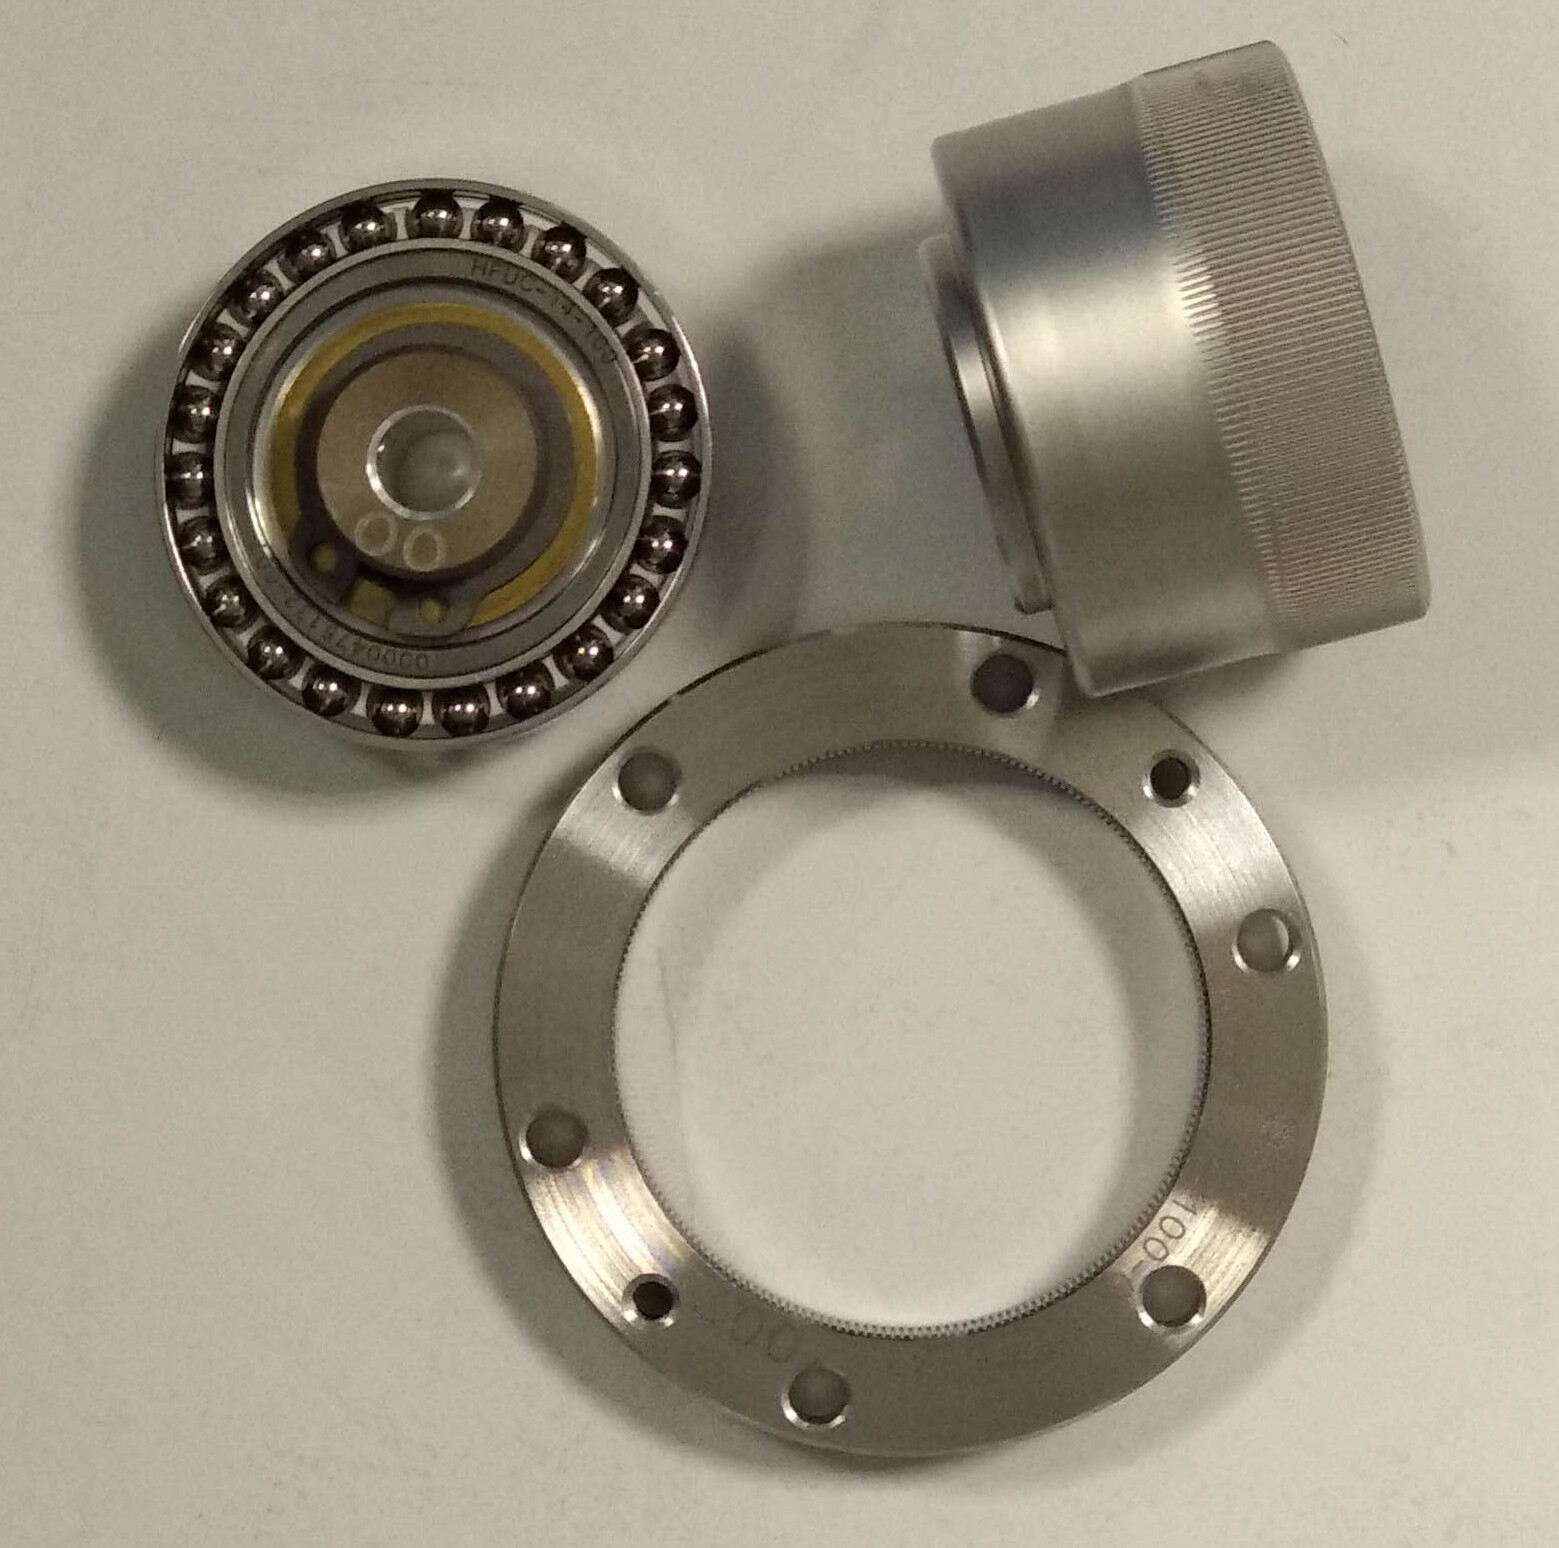
\includegraphics[width=\linewidth,height=3.2cm,keepaspectratio]{../../figures/d1_harmonic_drive.jpg}\\
\credit{Harmonic Drive strain-wave gear set. Pieceofmetalwork, CC BY-SA 4.0, via Wikimedia Commons}\\[1mm]
\begin{tikzpicture}[scale=.8,font=\scriptsize]
  \draw[thick,fill=mkPale] (0,0) rectangle (1.1,1.0) node[midway]{motor};
  \draw[thick,mkOrange,decorate,decoration={coil,aspect=.6,segment length=2mm,amplitude=1.6mm}] (1.1,.5) -- (2.6,.5);
  \node[mkOrange] at (1.85,1.0) {gear $k$};
  \draw[thick,fill=mkCream] (2.6,-.1) rectangle (4.0,1.1) node[midway]{arm};
\end{tikzpicture}
\end{columns}
\end{frame}

% ---------------------------------------------------------------------
\begin{frame}[t]{Refresher: natural frequency of a mass on a spring}
\begin{columns}[T,onlytextwidth]
\column{.40\textwidth}
\centering
\begin{tikzpicture}[font=\small]
  \fill[pattern=north east lines,pattern color=mkGray] (-1,3.2) rectangle (1,3.45);
  \draw[thick] (-1,3.2) -- (1,3.2);
  \draw[thick,mkOrange,decorate,decoration={coil,aspect=.6,segment length=2.5mm,amplitude=2.5mm}] (0,3.2) -- (0,1.6);
  \node[mkOrange,right] at (.35,2.4) {$k$};
  \draw[thick,fill=mkPale] (-.6,.8) rectangle (.6,1.6) node[midway]{$m$};
  \draw[{Latex}-{Latex},mkBlue,thick] (1.0,.7) -- (1.0,1.7) node[midway,right]{$x(t)$};
  \begin{scope}[xshift=2.6cm]
    \draw[thick] (-.6,3.3) -- (.6,3.3);
    \draw[mkGray,dashed] (0,3.3) -- (0,1.0);
    \draw[thick,mkNavy] (0,3.3) -- (-.8,1.3); \draw[thick,mkNavy] (0,3.3) -- (.8,1.3);
    \fill[mkOrange] (.8,1.3) circle (.12); \fill[mkOrange!40] (-.8,1.3) circle (.12);
    \node[below] at (0,.9) {swing};
  \end{scope}
\end{tikzpicture}
\begin{itemize}\small
\item Pull and let go: it oscillates at its \term{natural frequency}.
\item Push a swing in rhythm and it builds up: \term{resonance}.
\end{itemize}
\column{.56\textwidth}
\begin{eqbox}
\vspace{-2mm}
\[
\omega_n=\sqrt{\frac{k}{m}}\ \ [\si{rad/s}],\qquad f_n=\frac{\omega_n}{2\pi}\ \ [\si{Hz}]
\]
\vspace{-4mm}
\end{eqbox}
{\small $k$ stiffness [\si{N/m}], $m$ mass [\si{kg}]. Rotating joint: $k$ in \si{N.m/rad}, $J$ in \si{kg.m^2}.}
\begin{keybox}[Example]
\small
1.\ $m=\SI{1}{kg}$, $k=\SI{100}{N/m}$\\
2.\ $\omega_n=\sqrt{100/1}=\SI{10}{rad/s}$\\
3.\ $f_n=10/(2\pi)\approx\SI{1.6}{Hz}$
\end{keybox}
{\small Stiffer $\Rightarrow$ higher $f_n$; heavier $\Rightarrow$ lower $f_n$.}
\end{columns}
\end{frame}

% ---------------------------------------------------------------------
\begin{frame}[t]{The two-mass model and its two special frequencies}
\begin{columns}[T,onlytextwidth]
\column{.47\textwidth}
\centering
\begin{tikzpicture}[font=\scriptsize,scale=.92]
  \draw[thick,fill=mkPale] (0,0) rectangle (1.2,1.2) node[midway]{$J_M$};
  \draw[thick,fill=mkCream] (3.4,0) rectangle (4.6,1.2) node[midway]{$J_L$};
  \draw[thick,mkOrange,decorate,decoration={coil,aspect=.6,segment length=2mm,amplitude=1.6mm}] (1.2,.6) -- (3.4,.6);
  \node[above] at (2.3,.8) {$k$};
  \draw[sig,mkOrange] (-.9,.6) -- (0,.6) node[pos=0,left]{$T_M$};
  \node[mkBlue] at (.6,1.5) {motor};
  \node[mkBlue] at (4.0,1.5) {load (arm)};
\end{tikzpicture}
\begin{eqbox}
\vspace{-2mm}
\[
\omega_\text{AR}=\sqrt{\frac{k}{J_L}},\qquad
\omega_\text{R}=\omega_\text{AR}\sqrt{1+R}
\]
\vspace{-5mm}
\[ R=J_L/J_M \ \text{(inertia ratio)} \]
\vspace{-4mm}
\end{eqbox}
\begin{itemize}\small
\item \term{Anti-resonance} (AR): the load swings, the motor stands still.
\item \term{Resonance} (R): motor and load swing against each other.
\end{itemize}
\column{.5\textwidth}
\begin{keybox}[Worked example]
\small
1.\ $J_M=\SI{1.2e-4}{kg.m^2}$, $J_L=\SI{6e-4}{kg.m^2}$, $k=\SI{600}{N.m/rad}$\\[1mm]
2.\ $\omega_\text{AR}=\sqrt{600/(6\cdot10^{-4})}=\SI{1000}{rad/s}$ $\Rightarrow f_\text{AR}=\SI{159}{Hz}$\\[1mm]
3.\ $R=6/1.2=5$, $\sqrt{1+R}=2.45$\\[1mm]
4.\ $\omega_\text{R}=\SI{2449}{rad/s}$ $\Rightarrow f_\text{R}=\SI{390}{Hz}$
\end{keybox}
\gofurther{Newton's law for each inertia with shaft torque $T_S=k(\theta_M-\theta_L)+c(\omega_M-\omega_L)$ gives the full transfer functions; through a gear $N$ the load appears as $J_L/N^2$, $k/N^2$.}
\end{columns}
\end{frame}

% ---------------------------------------------------------------------
\begin{frame}[t]{What resonance looks like in time: a short torque push}
\begin{columns}[T,onlytextwidth]
\column{.6\textwidth}
\centering
\begin{tikzpicture}
\begin{axis}[mkplot,width=\linewidth,height=5.6cm,xmin=0,xmax=30,ymin=0,ymax=4.5,
  xlabel={time $t$ [ms]},ylabel={speed [rad/s]},legend pos=north east]
\addplot[mkBlue,thick] table[x=t,y=wM]{\dat{tm_time}};
\addplot[mkOrange,thick] table[x=t,y=wL]{\dat{tm_time}};
\addplot[mkGray,dashed,domain=0:30,samples=2]{2.5};
\legend{motor $\omega_M$, load $\omega_L$, rigid body}
\fill[mkSky,opacity=.25] (axis cs:0,0) rectangle (axis cs:5,4.5);
\node[font=\tiny,mkNavy] at (axis cs:2.5,4.2) {torque on};
\end{axis}
\end{tikzpicture}
\column{.38\textwidth}
\begin{itemize}\small
\item Same two-mass system: \SI{0.36}{N.m} for \SI{5}{ms}.
\item A rigid body would just ramp up to \SI{2.5}{rad/s} and stay there.
\item Here motor and load \hl{swap energy} through the spring at $f_\text{R}=\SI{390}{Hz}$ (period \SI{2.6}{ms}).
\item Low damping $\Rightarrow$ the ringing dies out slowly.
\end{itemize}
\begin{notebox}
\small The encoder sits on the motor: the controller sees the blue curve, but the \hl{tool} follows the orange one.
\end{notebox}
\end{columns}
\end{frame}

% ---------------------------------------------------------------------
\begin{frame}[t]{Frequency response of the two-mass system}
\begin{columns}[T,onlytextwidth]
\column{.6\textwidth}
\centering
\begin{tikzpicture}
\begin{axis}[mkplot,width=\linewidth,height=6.1cm,xmode=log,xmin=10,xmax=3000,ymin=-30,ymax=40,
  xlabel={frequency $f$ [Hz]},ylabel={motor speed per torque [dB]},
  legend pos=south west]
\addplot[mkSky,thick,dashed] table[x=f,y=r5]{\dat{twomass}};
\addplot[mkBlue,thick] table[x=f,y=G5]{\dat{twomass}};
\legend{rigid load, flexible (two-mass)}
\draw[mkOrange,thick,-{Latex}] (axis cs:159,-18) -- (axis cs:159,-4) node[pos=0,below,font=\scriptsize]{$f_\text{AR}=159$ Hz};
\draw[mkOrange,thick,-{Latex}] (axis cs:390,28) -- (axis cs:390,17) node[pos=0,above,font=\scriptsize]{$f_\text{R}=390$ Hz};
\end{axis}
\end{tikzpicture}
\column{.38\textwidth}
\begin{itemize}\small
\item Low $f$: motor and load move as one body.
\item Dip at $f_\text{AR}$, sharp \hl{peak} at $f_\text{R}$.
\item Above $f_\text{R}$ only the motor moves: gain $1+R=6\times$ ($\approx\SI{15.6}{dB}$) higher.
\item Large inertia ratio $R$ $\Rightarrow$ bigger jump, harder tuning.
\end{itemize}
\begin{notebox}
\small Refresher: $\text{dB}=20\log_{10}|G|$; $+20$ dB $=\times10$, $+6$ dB $\approx\times2$.
\end{notebox}
\end{columns}
\end{frame}

% ---------------------------------------------------------------------
\begin{frame}[t]{What the velocity loop sees}
\begin{columns}[T,onlytextwidth]
\column{.6\textwidth}
\centering
\begin{tikzpicture}
\begin{groupplot}[group style={group size=1 by 2,vertical sep=3mm,xticklabels at=edge bottom},
  mkplot,width=\linewidth,xmode=log,xmin=10,xmax=3000]
\nextgroupplot[height=3.9cm,ymin=-40,ymax=30,ylabel={loop gain [dB]},legend pos=north east,legend columns=3]
\addplot[mkSky,thick,dashed] table[x=f,y=Lr]{\dat{velloop}};
\addplot[mkRed,thick] table[x=f,y=L0]{\dat{velloop}};
\addplot[mkBlue,thick] table[x=f,y=L1]{\dat{velloop}};
\addplot[mkGray,thin,domain=10:3000,samples=2]{0};
\legend{rigid, two-mass, + notch}
\nextgroupplot[height=3.0cm,ymin=-300,ymax=90,ytick={-270,-180,-90,0,90},ylabel={phase [$^\circ$]},xlabel={frequency $f$ [Hz]}]
\addplot[mkSky,thick,dashed] table[x=f,y=pr]{\dat{velloop}};
\addplot[mkRed,thick] table[x=f,y=p0]{\dat{velloop}};
\addplot[mkBlue,thick] table[x=f,y=p1]{\dat{velloop}};
\addplot[mkGray,thin,domain=10:3000,samples=2]{-180};
\end{groupplot}
\end{tikzpicture}
\column{.38\textwidth}
\small Velocity loop tuned for \SI{50}{Hz} bandwidth, load from the example.
\begin{itemize}\small
\item Red: the resonance lifts the loop gain \hl{above 0 dB} at \SI{390}{Hz} $\Rightarrow$ the axis rings.
\item Blue: a \term{notch filter} at \SI{390}{Hz} pushes the peak back down below 0 dB.
\item Price: a little phase lost at \SI{50}{Hz} (about $9^\circ$).
\end{itemize}
\end{columns}
\end{frame}

% ---------------------------------------------------------------------
\begin{frame}[t]{The notch filter: cutting out one frequency}
\begin{columns}[T,onlytextwidth]
\column{.6\textwidth}
\centering
\begin{tikzpicture}
\begin{groupplot}[group style={group size=1 by 2,vertical sep=3mm,xticklabels at=edge bottom},
  mkplot,width=\linewidth,xmode=log,xmin=50,xmax=3000]
\nextgroupplot[height=3.6cm,ymin=-45,ymax=3,ylabel={gain [dB]},legend pos=south west]
\addplot[mkOrange,thick] table[x=f,y=m2]{\dat{notch}};
\addplot[mkSky,thick,dashed] table[x=f,y=m3]{\dat{notch}};
\legend{wide notch, narrow notch}
\nextgroupplot[height=2.9cm,ymin=-95,ymax=95,ytick={-90,0,90},ylabel={phase [$^\circ$]},xlabel={frequency $f$ [Hz], centre $f_n=\SI{400}{Hz}$}]
\addplot[mkOrange,thick] table[x=f,y=p2]{\dat{notch}};
\addplot[mkSky,thick,dashed] table[x=f,y=p3]{\dat{notch}};
\end{groupplot}
\end{tikzpicture}
\column{.38\textwidth}
\begin{itemize}\small
\item A \term{notch} (band-stop) filter removes a narrow band around $f_n$ and passes everything else at 0 dB.
\item It sits in the torque (current) command, after the velocity controller.
\item \term{Depth}: how much it cuts. \term{Width}: how many Hz it covers.
\item Wide = robust if $f_\text{R}$ drifts, but costs more phase at low $f$.
\end{itemize}
\gofurther{biquad $N(s)=\dfrac{s^2+2\zeta_z\omega_n s+\omega_n^2}{s^2+2\zeta_p\omega_n s+\omega_n^2}$, depth $\zeta_z/\zeta_p$; Tustin discretisation (W1D4).}
\end{columns}
\end{frame}

% ---------------------------------------------------------------------
\begin{frame}[t]{Notch or low-pass? Setting up the filter}
\begin{columns}[T,onlytextwidth]
\column{.5\textwidth}
\centering
\begin{tikzpicture}
\begin{axis}[mkplot,width=\linewidth,height=4.2cm,xmode=log,xmin=10,xmax=5000,ymin=-30,ymax=3,
  ylabel={gain [dB]},xlabel={frequency $f$ [Hz]},legend pos=south west]
\addplot[mkBlue,thick] table[x=f,y=m2]{\dat{lpf}};
\legend{{2nd-order LPF (corner 1 kHz)}}
\draw[mkOrange,thick,dashed] (axis cs:390,-30) -- (axis cs:390,3);
\node[font=\tiny,mkOrange,anchor=west] at (axis cs:400,-20) {$f_\text{R}$};
\end{axis}
\end{tikzpicture}
{\small A \term{low-pass filter} (LPF) is good against \hl{broad} high-frequency noise, but at \SI{390}{Hz} a \SI{1}{kHz} LPF cuts almost nothing.}
\column{.47\textwidth}
\begin{enumerate}\small
\item Measure the frequency response at low gain (sine sweep / chirp).
\item Read $f_\text{R}$ from the peak; check it at several arm poses and payloads.
\item Set $f_n=f_\text{R}$, depth \SIrange{10}{20}{dB}.
\item Widen it if $f_\text{R}$ moves by more than about $\pm10\,\%$.
\item Raise the velocity gain again and re-check the margins.
\end{enumerate}
\begin{keybox}[Rule of thumb]
\small Keep $f_n\gtrsim(3$--$5)\,f_c$. If the resonance is too close to the loop bandwidth, no filter helps: stiffen the mechanics or lower $f_c$.
\end{keybox}
\end{columns}
\end{frame}

% ---------------------------------------------------------------------
\begin{frame}[t]{Robot joints: the resonance moves with pose and payload}
\begin{columns}[T,onlytextwidth]
\column{.5\textwidth}
\centering
\begin{tikzpicture}
\begin{axis}[mkplot,width=\linewidth,height=4.6cm,xmin=0,xmax=10,ymin=5,ymax=28,
  xlabel={payload $m$ at \SI{0.8}{m} [kg]},ylabel={frequency [Hz]},legend pos=north east]
\addplot[mkOrange,thick] table[x=m,y=fR]{\dat{fr_payload}};
\addplot[mkBlue,thick,dashed] table[x=m,y=fAR]{\dat{fr_payload}};
\legend{$f_\text{R}$ resonance, $f_\text{AR}$ anti-resonance}
\end{axis}
\end{tikzpicture}
{\scriptsize Joint with harmonic gear $N=100$, joint stiffness \SI{2e4}{N.m/rad}.}
\column{.47\textwidth}
\begin{keybox}[Worked example: robot shoulder]
\small
1.\ Motor $J_m=\SI{1.5e-4}{kg.m^2}$ seen at the joint: $J_mN^2=\SI{1.5}{kg.m^2}$\\
2.\ Arm $J_L=\SI{2}{kg.m^2}$, $k=\SI{2e4}{N.m/rad}$\\
3.\ $f_\text{AR}=\frac{1}{2\pi}\sqrt{2\cdot10^4/2}=\SI{15.9}{Hz}$\\
4.\ $R=2/1.5=1.33$, $f_\text{R}=15.9\sqrt{2.33}=\SI{24.3}{Hz}$
\end{keybox}
\begin{itemize}\small
\item Robot resonances are \hl{low} (\SIrange{5}{30}{Hz}) and change with reach and payload.
\item Hence: robust (wide) notches, gain scheduling, input shaping.
\end{itemize}
\end{columns}
\end{frame}

% ---------------------------------------------------------------------
\begin{frame}[t]{Check your understanding -- 3.7}
\vspace{4mm}
\begin{keybox}[Check your understanding]
\large
\begin{enumerate}
\item The load inertia $J_L$ is made 4 times larger. What happens to $f_\text{AR}$?\\[2mm]
\item The velocity-loop bandwidth is \SI{50}{Hz}, the resonance is at \SI{390}{Hz}. Why a notch and not a low-pass filter?\\[2mm]
\item The robot picks up a heavy part. Does its joint resonance go up or down?
\end{enumerate}
\end{keybox}
\vfill
\centering\small\color{mkGray} Discuss with your neighbour for 2 minutes.
\end{frame}

% ---------------------------------------------------------------------
\begin{frame}[t]{Summary 3.7 -- Resonance and notch filters}
\begin{columns}[T,onlytextwidth]
\column{.55\textwidth}
\begin{keybox}[Key take-aways]
\small
\begin{itemize}
\item A compliant joint = motor inertia + spring + load inertia.
\item $f_\text{AR}=\frac1{2\pi}\sqrt{k/J_L}$, $f_\text{R}=f_\text{AR}\sqrt{1+R}$.
\item The resonance peak can lift the loop gain above 0 dB $\Rightarrow$ ringing.
\item \hl{Notch} for one narrow peak, \hl{LPF} for broad noise.
\item In robots $f_\text{R}$ changes with pose and payload: fix the mechanics first, filter second.
\end{itemize}
\end{keybox}
\column{.42\textwidth}
\begin{defbox}[Key terms]
\small
\term{compliance} springiness of a part\\
\term{natural frequency} rate of free oscillation\\
\term{anti-resonance} dip: motor still\\
\term{resonance} peak: masses swing apart\\
\term{inertia ratio} $R=J_L/J_M$\\
\term{notch} narrow band-stop filter
\end{defbox}
{\scriptsize\color{mkGray} [Ellis, 2012]; [Spong et al., 2020, ch.~6].}
\end{columns}
\end{frame}

% =====================================================================
\section[4.1 Robot anatomy]{4.1 Robot Anatomy and Classification}
% =====================================================================

\begin{frame}[t]{Anatomy of a robot arm}
\begin{columns}[T,onlytextwidth]
\column{.5\textwidth}
\centering
\begin{tikzpicture}[scale=.95,font=\scriptsize]
  \fill[pattern=north east lines,pattern color=mkGray] (-1.2,-.25) rectangle (1.2,0);
  \draw[thick] (-1.2,0) -- (1.2,0);
  \draw[thick,fill=mkPale] (-.5,0) rectangle (.5,.6);
  \node[joint] (j1) at (0,.6) {};
  \draw[link] (0,.6) -- (0,1.5);
  \node[joint] (j2) at (0,1.5) {};
  \draw[link] (0,1.5) -- (1.6,2.7);
  \node[joint] (j3) at (1.6,2.7) {};
  \draw[link] (1.6,2.7) -- (3.0,2.2);
  \node[joint] (j4) at (3.0,2.2) {};
  \draw[thick,mkOrange] (3.0,2.2) -- (3.3,1.8);
  \draw[thick,mkOrange] (3.15,1.6) -- (3.45,2.0) (3.15,1.6) -- (3.05,1.45) (3.45,2.0) -- (3.6,1.9);
  \node[lbl,anchor=east] at (-.6,.3) {base};
  \node[lbl,anchor=east] at (-.15,1.5) {shoulder};
  \node[lbl,anchor=south] at (1.6,2.8) {elbow};
  \node[lbl,anchor=south] at (3.1,2.3) {wrist};
  \node[lbl,anchor=north,mkOrange] at (3.35,1.4) {end-effector};
  \node[lbl,anchor=north west] at (.8,1.9) {link};
  \draw[mkMid,dashed] (0,.6) circle (.35);
\end{tikzpicture}
\column{.47\textwidth}
\begin{itemize}\small
\item \term{Links}: the rigid bodies (``bones'').
\item \term{Joints}: connect links and allow motion (``body joints''); each has a motor.
\item \term{Base}: fixed to the floor; \term{wrist}: orients the tool.
\item \term{End-effector} (EOAT): gripper, welding torch, suction cup (W1D2).
\item Serial chain: base -- link -- joint -- link -- \ldots -- tool.
\end{itemize}
\begin{notebox}
\small Analogy: your own arm. Shoulder (3 rotations), elbow (1), wrist (3): about 7 joints.
\end{notebox}
\end{columns}
\end{frame}

% ---------------------------------------------------------------------
\begin{frame}[t]{Joint types: revolute and prismatic}
\begin{columns}[T,onlytextwidth]
\column{.5\textwidth}
\centering
\begin{tikzpicture}[font=\scriptsize]
  % revolute
  \draw[link] (0,0) -- (1.2,0);
  \node[circle,draw=mkNavy,fill=white,thick,minimum size=6mm] at (1.2,0) {};
  \fill[mkNavy] (1.2,0) circle (.06);
  \draw[link,mkOrange] (1.2,0) -- (2.2,.8);
  \draw[-{Latex},thick,mkOrange] (1.95,.05) arc (0:38:.75);
  \node[mkOrange] at (2.25,.25) {$\theta$};
  \node[mkNavy,font=\small\bfseries] at (1.1,-.8) {Revolute (R)};
  \node[lbl] at (1.1,-1.15) {rotation, variable $\theta$ [rad]};
  % prismatic
  \begin{scope}[xshift=3.2cm]
    \draw[thick,fill=mkPale] (0,-.25) rectangle (1.5,.25);
    \draw[thick,fill=mkCream] (.9,-.15) rectangle (2.4,.15);
    \draw[{Latex}-{Latex},thick,mkOrange] (.9,.45) -- (2.4,.45) node[midway,above]{$d$};
    \node[mkNavy,font=\small\bfseries] at (1.2,-.8) {Prismatic (P)};
    \node[lbl] at (1.2,-1.15) {sliding, variable $d$ [m]};
  \end{scope}
\end{tikzpicture}\\[3mm]
\small Both have \hl{1 degree of freedom}. Others (spherical = 3, universal = 2) are made from R joints.
\column{.47\textwidth}
\begin{defbox}[Joint variable]
\small The one number that says where a joint is: angle $\theta_i$ (R) or stroke $d_i$ (P). All of them together form the \term{joint vector} $\bm q=(q_1,\ldots,q_n)$.
\end{defbox}
\begin{itemize}\small
\item Robots are named by their joint string, base to wrist: e.g.\ \textbf{RRP} for a SCARA's first three, \textbf{PPP} for a gantry.
\item The motor and encoder of W1 sit in every joint.
\end{itemize}
\end{columns}
\end{frame}

% ---------------------------------------------------------------------
\begin{frame}[t]{Degrees of freedom (DOF)}
\begin{columns}[T,onlytextwidth]
\column{.5\textwidth}
\begin{itemize}\small
\item A free body in space has \hl{6 DOF}: 3 positions $(x,y,z)$ + 3 orientations (roll, pitch, yaw).
\item In a plane: 3 DOF $(x,y,\varphi)$.
\item To place a tool at \emph{any} position \emph{and} orientation, a robot needs \hl{6 joints}.
\item 7+ joints: \term{redundant} (like your arm): it can move the elbow while the hand stays still.
\end{itemize}
\begin{tikzpicture}[scale=.8,font=\scriptsize,x={(1cm,0cm)},y={(.5cm,.35cm)},z={(0cm,1cm)}]
  \draw[ax,mkOrange] (0,0,0) -- (1.6,0,0) node[right]{$x$};
  \draw[ax,mkMid] (0,0,0) -- (0,1.8,0) node[above right]{$y$};
  \draw[ax,mkBlue] (0,0,0) -- (0,0,1.4) node[above]{$z$};
  \draw[-{Latex},mkOrange] (1.1,-.2,-.25) arc (-90:200:.12 and .3);
  \node[mkGray] at (3.2,0,.6) {3 translations + 3 rotations};
\end{tikzpicture}
\column{.47\textwidth}
\begin{defbox}[Counting mobility (Grübler)]
\small Planar: $M=3(n-1)-2j$, \quad $n$ links incl.\ ground, $j$ one-DOF joints.
\end{defbox}
\begin{keybox}[Worked example]
\small
1.\ Planar 2-link arm: $n=3$, $j=2$\\
\phantom{1.\ }$M=3\cdot2-2\cdot2=2$\\
2.\ Four-bar linkage: $n=4$, $j=4$\\
\phantom{2.\ }$M=3\cdot3-2\cdot4=1$\\
3.\ Spatial 6-axis arm: $M=6\cdot6-5\cdot6=6$
\end{keybox}
\end{columns}
\end{frame}

% ---------------------------------------------------------------------
\begin{frame}[t]{Workspace: where can the tool reach?}
\begin{columns}[T,onlytextwidth]
\column{.48\textwidth}
\centering
\begin{tikzpicture}[scale=3.2,font=\scriptsize]
  \fill[mkSky!30,even odd rule] (0,0) circle (.7) (0,0) circle (.1);
  \draw[mkBlue,thick] (0,0) circle (.7); \draw[mkBlue,thick] (0,0) circle (.1);
  \draw[gray!50,->] (-.8,0) -- (.85,0) node[right]{$x$};
  \draw[gray!50,->] (0,-.8) -- (0,.85) node[above]{$y$};
  \draw[link,line width=2pt] (0,0) -- (30:.4) -- ($(30:.4)+(90:.3)$);
  \node[joint,minimum size=1.8mm] at (0,0) {}; \node[joint,minimum size=1.8mm] at (30:.4) {};
  \fill[mkOrange] ($(30:.4)+(90:.3)$) circle (.025);
  \draw[{Latex}-{Latex},mkOrange] (0,0) -- (-45:.7) node[midway,below left]{$\ell_1+\ell_2$};
  \draw[{Latex}-{Latex},mkNavy] (0,0) -- (200:.1);
  \node[mkNavy] at (205:.25) {$|\ell_1-\ell_2|$};
\end{tikzpicture}
\column{.5\textwidth}
\begin{itemize}\small
\item \term{Workspace}: the set of all points the tool can reach.
\item \term{Dexterous workspace}: points reachable with \emph{any} orientation (smaller).
\item Planar 2-link with full joint range: a ring between $|\ell_1-\ell_2|$ and $\ell_1+\ell_2$.
\end{itemize}
\begin{keybox}[Example]
\small $\ell_1=\SI{0.4}{m}$, $\ell_2=\SI{0.3}{m}$: inner radius \SI{0.1}{m}, outer \SI{0.7}{m}. A part at \SI{0.75}{m} is \hl{out of reach}; move the robot or the part.
\end{keybox}
{\scriptsize Real joints have limits (cables, collisions), so the true workspace is smaller than the ring.}
\end{columns}
\end{frame}

% ---------------------------------------------------------------------
\begin{frame}[t]{Articulated arms and SCARA robots}
\begin{columns}[T,onlytextwidth]
\column{.49\textwidth}
\centering
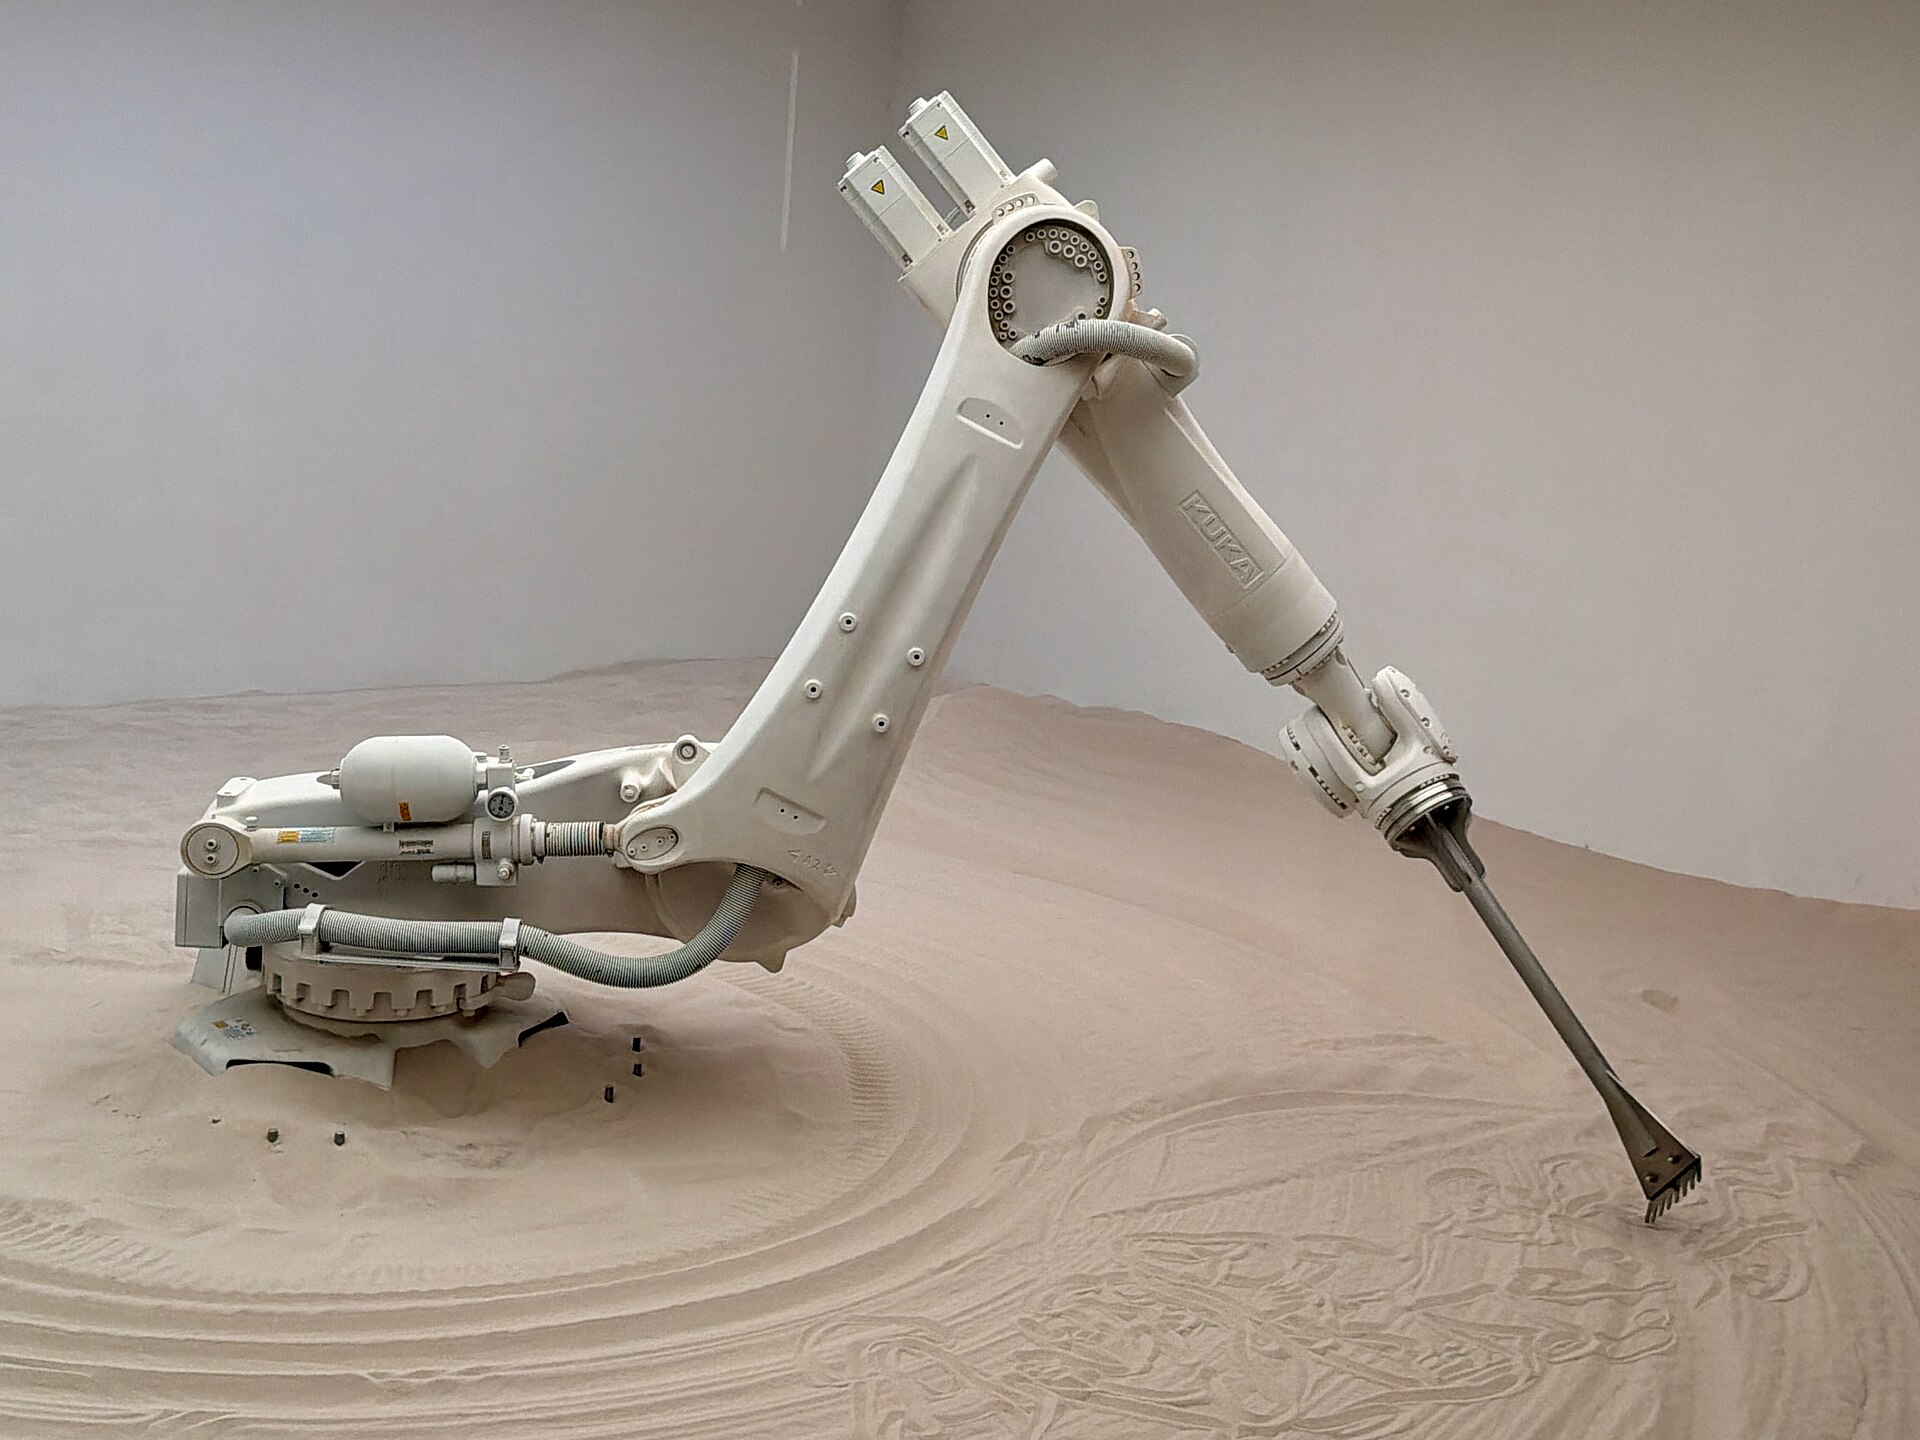
\includegraphics[width=\linewidth,height=3.4cm,keepaspectratio]{../../figures/d4_kuka_robot.jpg}\\
\credit{KUKA industrial arm. Oleg Yunakov, CC BY-SA 4.0, via Wikimedia Commons}\\[1mm]
\begin{itemize}\small
\item \term{Articulated} (6R): like a human arm; large spherical workspace.
\item Welding, painting, machine tending, palletising.
\end{itemize}
\column{.49\textwidth}
\centering
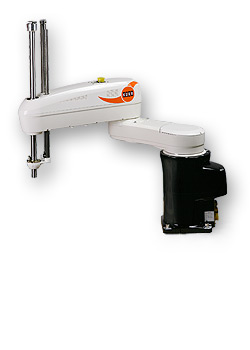
\includegraphics[width=\linewidth,height=3.4cm,keepaspectratio]{../../figures/r21_scara.jpg}\\
\credit{KUKA KR10 SCARA. Jo Teichmann, Public domain, via Wikimedia Commons}\\[1mm]
\begin{itemize}\small
\item \term{SCARA} (RRPR): two vertical-axis R joints, one vertical P, one tool rotation.
\item Stiff vertically, compliant sideways: fast pick-and-place, assembly.
\end{itemize}
\end{columns}
\end{frame}

% ---------------------------------------------------------------------
\begin{frame}[t]{Cartesian / gantry and delta (parallel) robots}
\begin{columns}[T,onlytextwidth]
\column{.49\textwidth}
\centering
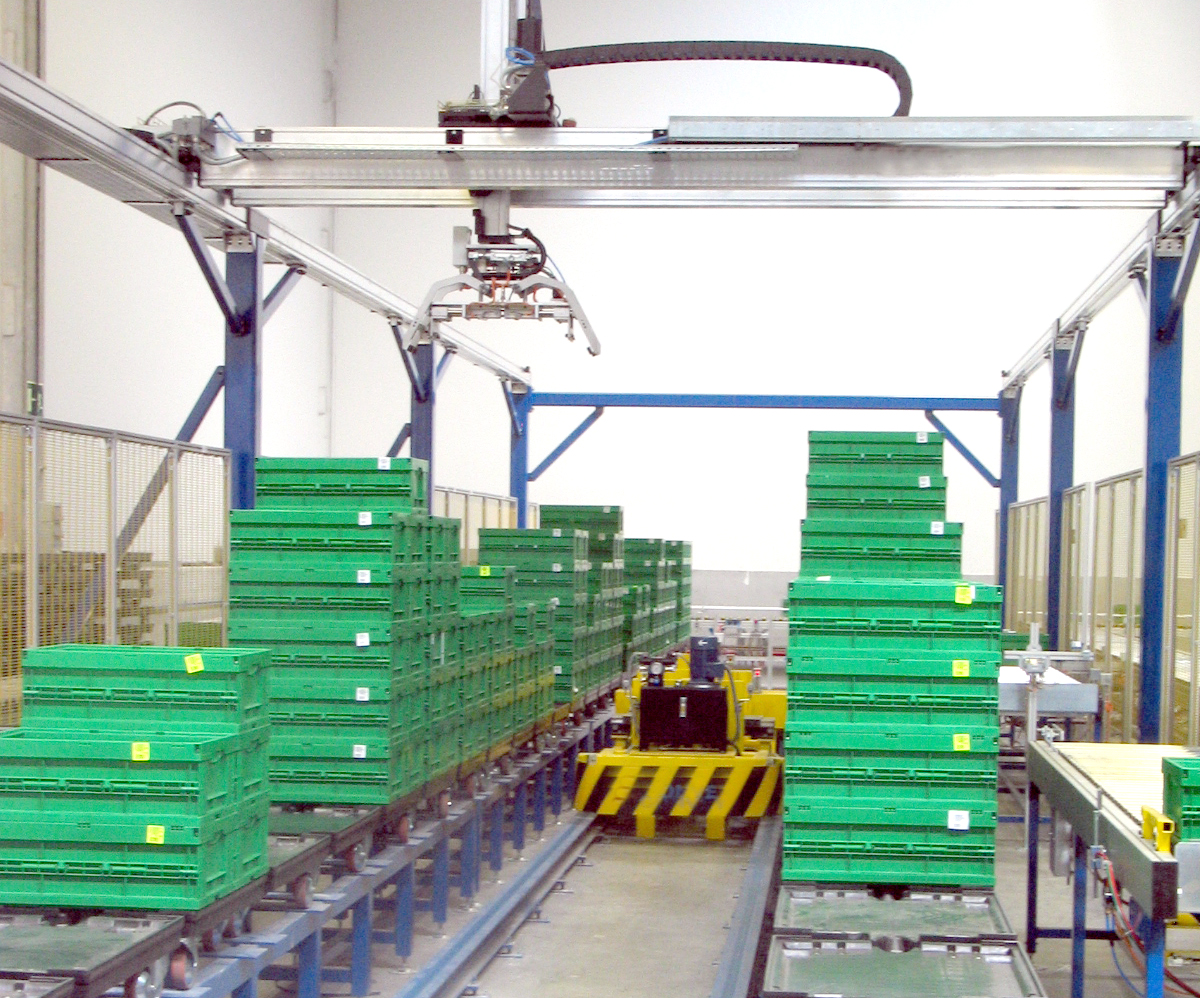
\includegraphics[width=\linewidth,height=3.4cm,keepaspectratio]{../../figures/r21_gantry.jpg}\\
\credit{Gantry robot over a palletising line. www.tecnowey.com, CC BY 3.0, via Wikimedia Commons}\\[1mm]
\begin{itemize}\small
\item \term{Cartesian / gantry} (PPP): three linear axes, box-shaped workspace.
\item Simple kinematics, scalable size: 3D printers, CNC, large handling.
\end{itemize}
\column{.49\textwidth}
\centering
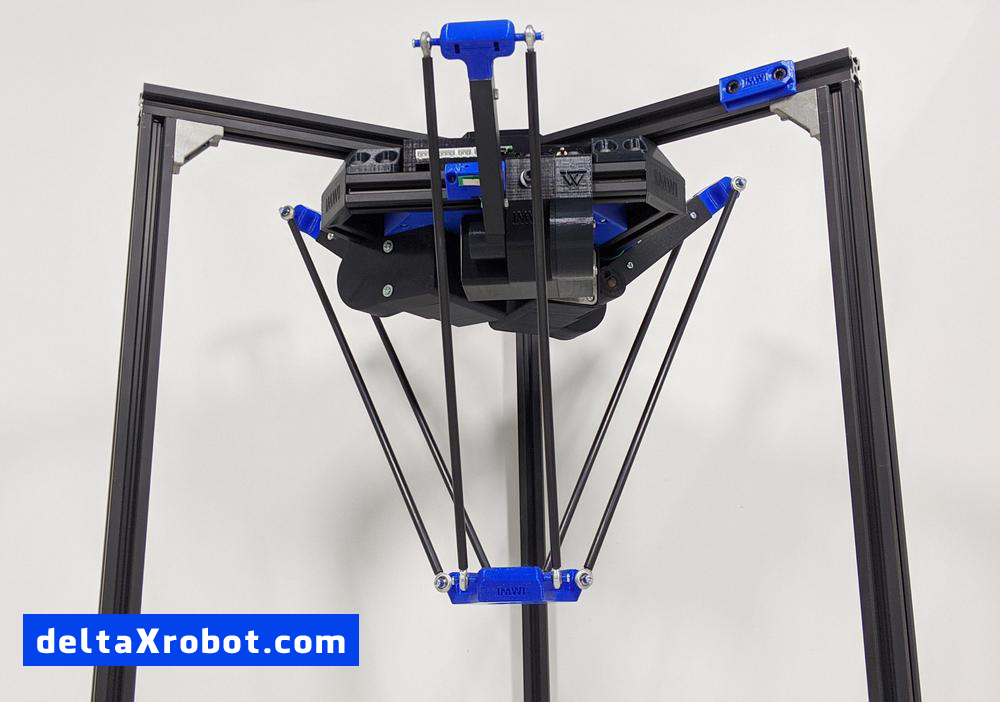
\includegraphics[width=\linewidth,height=3.4cm,keepaspectratio]{../../figures/r21_delta.jpg}\\
\credit{Delta X robot. Trungdoanhong, CC BY-SA 4.0, via Wikimedia Commons}\\[1mm]
\begin{itemize}\small
\item \term{Delta} (parallel): three arms share one light platform.
\item Motors stay on the base $\Rightarrow$ very fast picking (food, pharma).
\end{itemize}
\end{columns}
\end{frame}

% ---------------------------------------------------------------------
\begin{frame}[t]{Serial vs.\ parallel kinematic chains}
\begin{columns}[T,onlytextwidth]
\column{.48\textwidth}
\centering
\begin{tikzpicture}[font=\scriptsize]
  % serial
  \draw[thick] (-.4,0) -- (.4,0); \fill[pattern=north east lines,pattern color=mkGray] (-.4,-.15) rectangle (.4,0);
  \draw[link] (0,0) -- (.3,1.0) -- (1.1,1.5) -- (1.6,1.0);
  \foreach \p in {(0,0),(.3,1.0),(1.1,1.5)} \node[joint] at \p {};
  \fill[mkOrange] (1.6,1.0) circle (.07);
  \node[mkNavy,font=\small\bfseries] at (.7,-.5) {serial};
  % parallel
  \begin{scope}[xshift=3cm]
    \draw[thick] (-.9,1.9) -- (.9,1.9); \fill[pattern=north east lines,pattern color=mkGray] (-.9,1.9) rectangle (.9,2.05);
    \foreach \a/\b in {-.8/-.25,0/0,.8/.25}{
      \draw[link,line width=2pt] (\a,1.9) -- ({\a*1.3},1.0) -- (\b,.3);
      \node[joint,minimum size=1.8mm] at (\a,1.9) {};
      \node[joint,minimum size=1.8mm] at ({\a*1.3},1.0) {};}
    \draw[thick,fill=mkCream] (-.35,.2) rectangle (.35,.35);
    \fill[mkOrange] (0,.12) circle (.07);
    \node[mkNavy,font=\small\bfseries] at (0,-.5) {parallel (delta)};
  \end{scope}
\end{tikzpicture}
\column{.5\textwidth}
\footnotesize
\begin{tabularx}{\linewidth}{@{}l X X@{}}
\toprule
 & \textbf{Serial} & \textbf{Parallel}\\
\midrule
Chain & open, one path & closed loops\\
Workspace & large & small\\
Stiffness & lower (errors add) & high\\
Moving mass & motors ride along & motors on base\\
Speed & medium & very high\\
Kinematics & forward easy & inverse easy\\
\bottomrule
\end{tabularx}
\end{columns}
\end{frame}

% ---------------------------------------------------------------------
\begin{frame}[t]{Collaborative and mobile robots}
\begin{columns}[T,onlytextwidth]
\column{.49\textwidth}
\centering
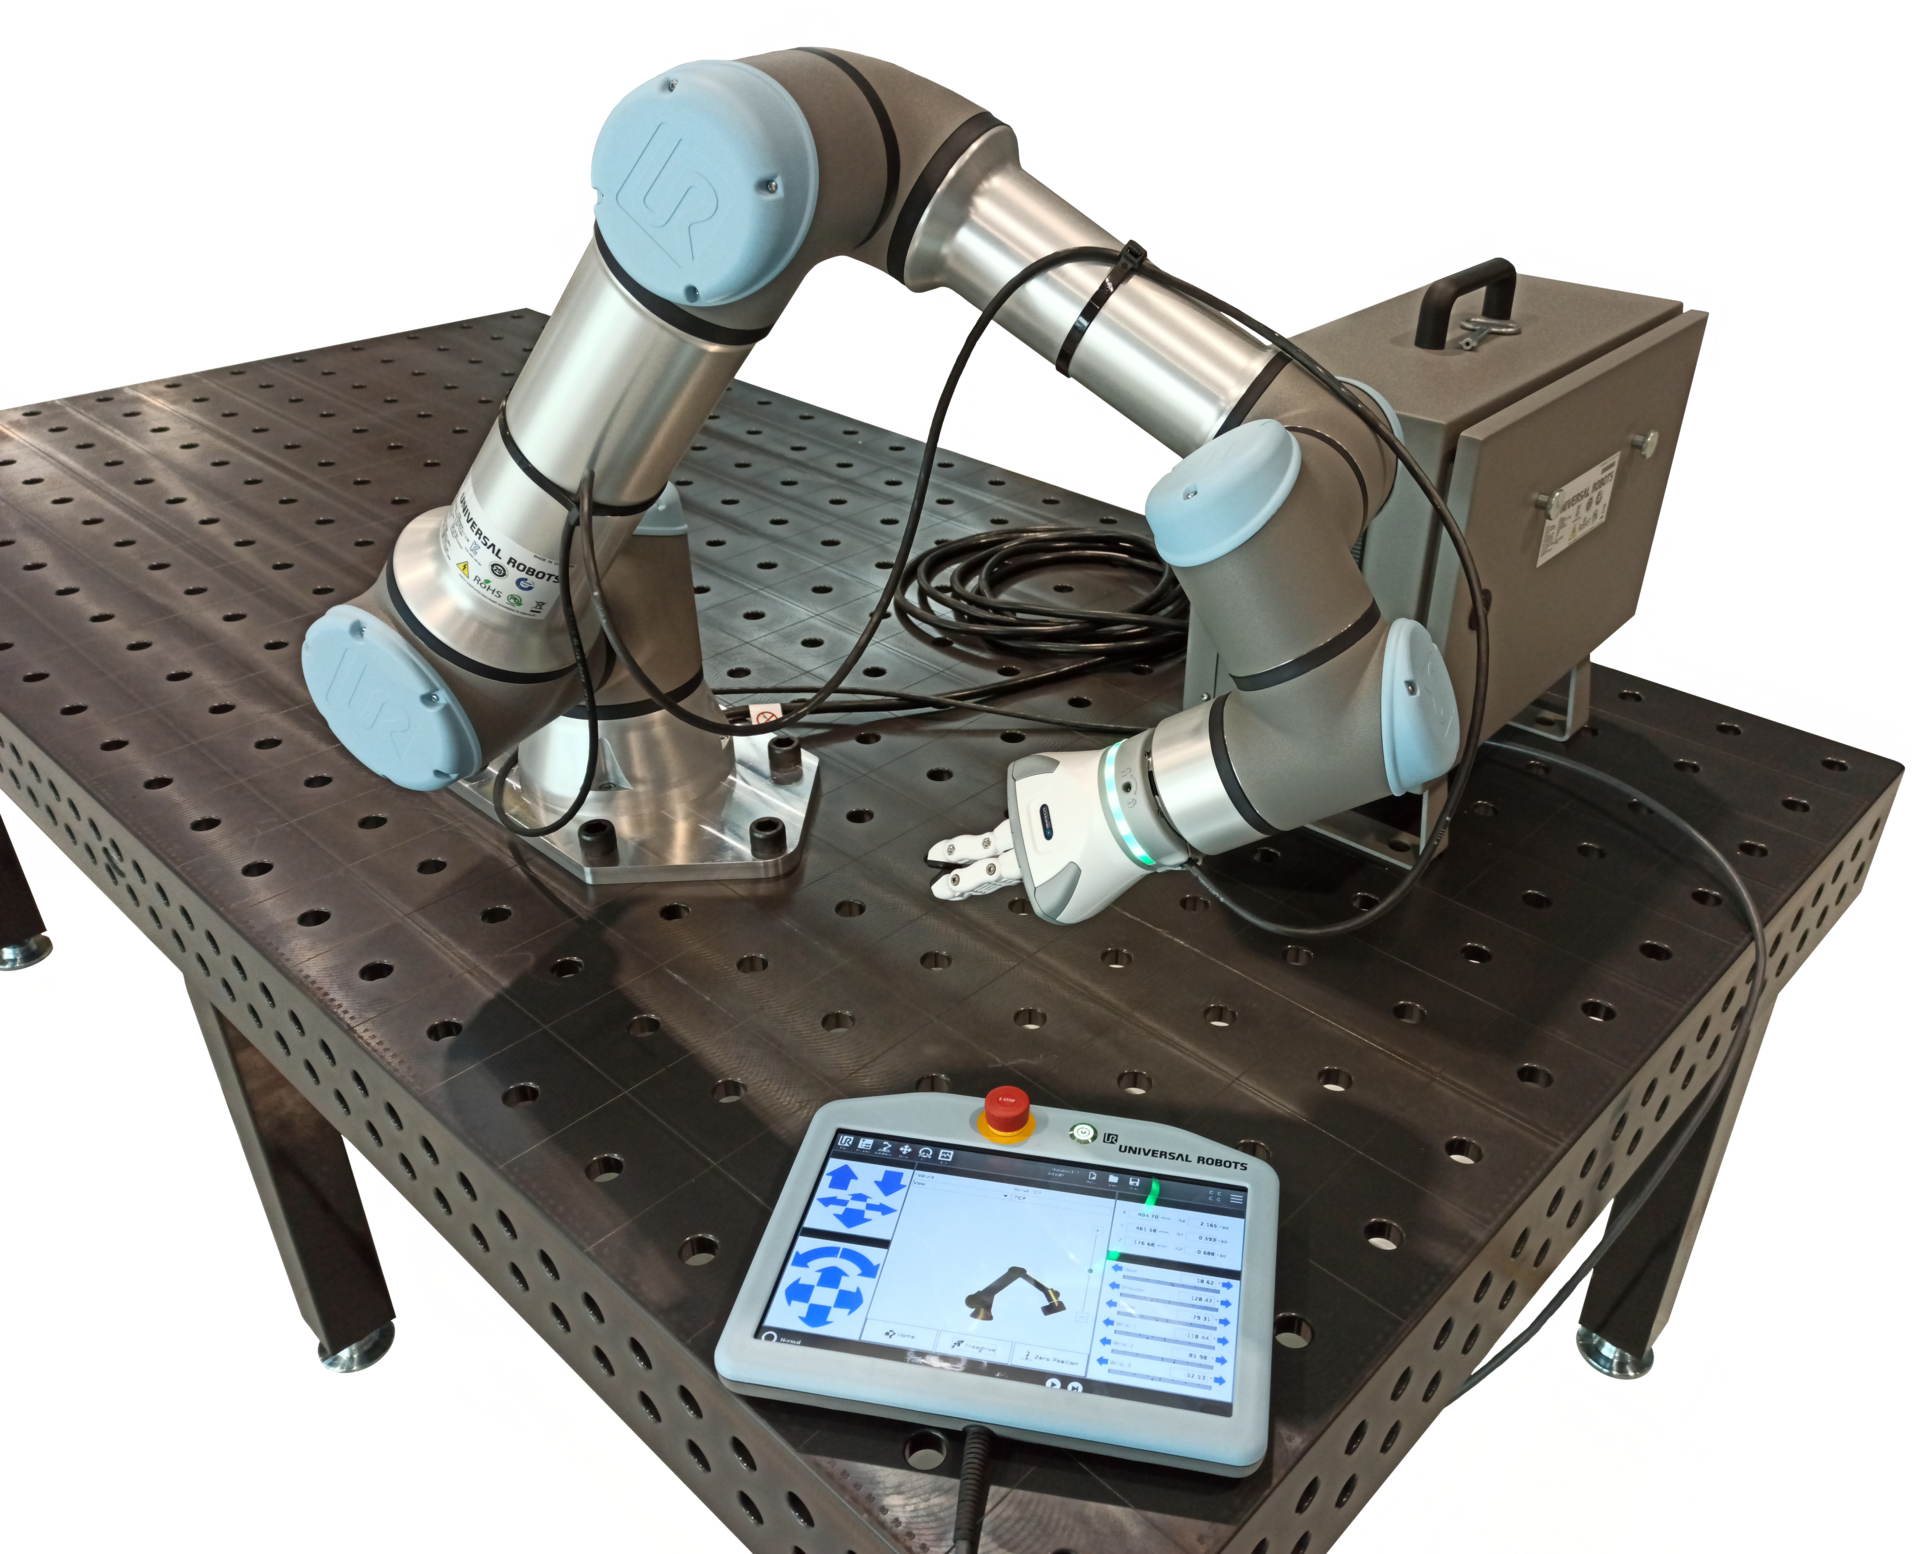
\includegraphics[width=\linewidth,height=3.3cm,keepaspectratio]{../../figures/r21_cobot.png}\\
\credit{UR16e cobot with teach pendant. Auledas, CC BY-SA 4.0, via Wikimedia Commons}\\[1mm]
\begin{itemize}\small
\item \term{Cobot}: light 6--7 axis arm made to work \hl{next to people}.
\item Joint torque sensing, speed and force limits (W2D4: ISO/TS 15066).
\end{itemize}
\column{.49\textwidth}
\centering

\includegraphics[width=\linewidth,height=3.3cm,keepaspectratio]{../../figures/r21_mobile.png}\\
\credit{Autonomous mobile robot (illustration). Rlistmedia, CC BY 4.0, via Wikimedia Commons}\\[1mm]
\begin{itemize}\small
\item \term{Mobile robot} (AGV / AMR): wheels instead of a fixed base.
\item Mobile manipulator = AMR + arm: the workspace travels.
\end{itemize}
\end{columns}
\end{frame}

% ---------------------------------------------------------------------
\begin{frame}[t]{Classification at a glance}
\centering
\footnotesize
\renewcommand{\arraystretch}{1.15}
\begin{tabularx}{\linewidth}{@{}l l l X X@{}}
\toprule
\textbf{Type} & \textbf{Joints} & \textbf{DOF} & \textbf{Workspace} & \textbf{Typical use}\\
\midrule
Articulated & RRRRRR & 6 & sphere-like & welding, painting, tending\\
SCARA & RRPR & 4 & cylinder & assembly, pick-and-place\\
Cartesian / gantry & PPP(R) & 3--4 & box & 3D printing, palletising, CNC loading\\
Delta & 3 parallel arms (+R) & 3--4 & small dome & high-speed picking\\
Cobot & 6--7 R & 6--7 & sphere-like & shared work with people\\
Mobile (AMR) & 2 driven wheels & 3 (plane) & the floor & logistics, intralogistics\\
\bottomrule
\end{tabularx}\\[3mm]
\begin{keybox}[How to choose]
\small Start from the task: \hl{reach} and workspace shape, \hl{payload}, \hl{speed}/cycle time, \hl{accuracy}, and whether people share the space (W2D3: work-cell design).
\end{keybox}
\end{frame}

% ---------------------------------------------------------------------
\begin{frame}[t]{Check your understanding -- 4.1}
\vspace{4mm}
\begin{keybox}[Check your understanding]
\large
\begin{enumerate}
\item How many joints does a robot need to place a tool at any position \emph{and} orientation in space?\\[2mm]
\item A planar arm has links $\ell_1=\SI{0.5}{m}$ and $\ell_2=\SI{0.5}{m}$. What is its workspace?\\[2mm]
\item Why is a delta robot faster than an articulated arm of similar size?
\end{enumerate}
\end{keybox}
\vfill
\centering\small\color{mkGray} Discuss with your neighbour for 2 minutes.
\end{frame}

% ---------------------------------------------------------------------
\begin{frame}[t]{Summary 4.1 -- Robot anatomy and classification}
\begin{columns}[T,onlytextwidth]
\column{.55\textwidth}
\begin{keybox}[Key take-aways]
\small
\begin{itemize}
\item A robot = links + joints (R or P) + base + end-effector.
\item 6 DOF to set position and orientation; more = redundant.
\item Workspace follows from link lengths and joint limits.
\item Serial: large workspace; parallel: stiff and fast.
\item Choose by reach, payload, speed, accuracy, people.
\end{itemize}
\end{keybox}
\column{.42\textwidth}
\begin{defbox}[Key terms]
\small
\term{link / joint} body / connection\\
\term{revolute, prismatic} rotate / slide\\
\term{DOF} independent motions\\
\term{workspace} reachable points\\
\term{SCARA, delta, gantry} robot types\\
\term{cobot, AMR} people-safe arm / mobile base
\end{defbox}
{\scriptsize\color{mkGray} [Craig, 2005, ch.~1]; [Siciliano et al., 2009, ch.~1].}
\end{columns}
\end{frame}

% =====================================================================
\section[4.2 Spatial descriptions]{4.2 Spatial Descriptions: Positions, Rotations, Homogeneous Transforms}
% =====================================================================

\begin{frame}[t]{Why we need coordinate frames}
\begin{columns}[T,onlytextwidth]
\column{.52\textwidth}
\centering
\begin{tikzpicture}[font=\scriptsize]
  \fill[pattern=north east lines,pattern color=mkGray] (-.6,-.15) rectangle (.6,0);
  \draw[link] (0,0) -- (.4,1.4) -- (2.0,1.9);
  \node[joint] at (0,0) {}; \node[joint] at (.4,1.4) {};
  \triad{0}{0}{0}{B}
  \triad{2.0}{1.9}{-60}{T}
  \draw[thick,fill=mkCream] (3.2,-.1) rectangle (4.6,.5);
  \triad{3.3}{.5}{0}{P}
  \node[mkGray] at (3.9,-.35) {part};
  \node[mkGray] at (-.2,-.5) {base $\{B\}$};
  \node[mkGray] at (2.3,2.4) {tool $\{T\}$};
\end{tikzpicture}
\column{.45\textwidth}
\begin{itemize}\small
\item Every object gets its own \term{frame}: an origin + 3 perpendicular axes.
\item \term{Base} frame $\{B\}$, \term{tool} frame $\{T\}$, part (user) frame $\{P\}$.
\item The camera sees the part in \emph{its} frame; the robot needs it in the base frame.
\item Task: describe one frame \hl{relative to another}.
\end{itemize}
\begin{notebox}
\small Analogy: ``two metres left of the door'' only makes sense if you know where the door is and which way you face.
\end{notebox}
\end{columns}
\end{frame}

% ---------------------------------------------------------------------
\begin{frame}[t]{Refresher: vectors and matrix--vector multiplication}
\begin{columns}[T,onlytextwidth]
\column{.48\textwidth}
\begin{defbox}[Refresher: matrix times vector]
\small Each output row = row of the matrix ``dotted'' with the vector:
\[
\begin{bmatrix}a&b\\c&d\end{bmatrix}\!\begin{bmatrix}x\\y\end{bmatrix}
=\begin{bmatrix}ax+by\\cx+dy\end{bmatrix}
\]
\end{defbox}
\begin{itemize}\small
\item A position vector ${}^A\bm p=(p_x,p_y,p_z)^T$: the point, measured in frame $\{A\}$.
\item The superscript says \hl{which frame} we measure in.
\end{itemize}
\column{.48\textwidth}
\begin{keybox}[Example]
\small
\[
\begin{bmatrix}0&-1\\1&0\end{bmatrix}\!\begin{bmatrix}2\\1\end{bmatrix}
=\begin{bmatrix}0\cdot2+(-1)\cdot1\\1\cdot2+0\cdot1\end{bmatrix}
=\begin{bmatrix}-1\\2\end{bmatrix}
\]
\end{keybox}
\centering
\begin{tikzpicture}[scale=.75,font=\scriptsize]
  \draw[gray!50,->] (-1.5,0) -- (2.5,0); \draw[gray!50,->] (0,-.3) -- (0,2.4);
  \draw[ax,mkBlue] (0,0) -- (2,1) node[right]{$(2,1)$};
  \draw[ax,mkOrange] (0,0) -- (-1,2) node[left]{$(-1,2)$};
  \draw[-{Latex},mkGray] (1.2,.6) arc (26.6:116.6:1.34);
  \node[mkGray] at (.75,1.55) {$90^\circ$};
\end{tikzpicture}\\
{\small This matrix rotates any vector by $90^\circ$.}
\end{columns}
\end{frame}

% ---------------------------------------------------------------------
\begin{frame}[t]{Rotation in the plane}
\begin{columns}[T,onlytextwidth]
\column{.45\textwidth}
\centering
\begin{tikzpicture}[scale=2.0,font=\scriptsize]
  \draw[ax,mkGray] (0,0) -- (1.3,0) node[right]{$x_A$};
  \draw[ax,mkGray] (0,0) -- (0,1.3) node[above]{$y_A$};
  \draw[ax,mkOrange] (0,0) -- (30:1.2) node[right]{$x_B$};
  \draw[ax,mkMid] (0,0) -- (120:1.2) node[above]{$y_B$};
  \draw[mkOrange] (.5,0) arc (0:30:.5); \node[mkOrange] at (15:.65) {$\theta$};
  \draw[mkOrange,dashed] (30:1) -- ({cos(30)},0) node[below]{$\cos\theta$};
  \draw[mkOrange,dashed] (30:1) -- (0,{sin(30)}) node[left]{$\sin\theta$};
\end{tikzpicture}
\column{.52\textwidth}
\begin{itemize}\small
\item Frame $\{B\}$ is turned by $\theta$ relative to $\{A\}$.
\item Unit vector $\hat x_B$ seen in $\{A\}$: $(\cos\theta,\sin\theta)$; $\hat y_B$: $(-\sin\theta,\cos\theta)$.
\item Put them side by side as \hl{columns}:
\end{itemize}
\begin{eqbox}
\vspace{-2mm}
\[
{}^A\!R_B(\theta)=\begin{bmatrix}\cos\theta&-\sin\theta\\ \sin\theta&\cos\theta\end{bmatrix},\qquad {}^A\bm p={}^A\!R_B\,{}^B\bm p
\]
\vspace{-4mm}
\end{eqbox}
\begin{keybox}[Example]
\small $\theta=30^\circ$, ${}^B\bm p=(1,0)$: ${}^A\bm p=(\cos30^\circ,\sin30^\circ)=(0.866,\,0.5)$.
\end{keybox}
\end{columns}
\end{frame}

% ---------------------------------------------------------------------
\begin{frame}[t]{Properties of rotation matrices}
\begin{columns}[T,onlytextwidth]
\column{.52\textwidth}
\begin{itemize}\small
\item \hl{Columns} = the axes of $\{B\}$ written in $\{A\}$.
\item Each column has length 1, columns are perpendicular: the matrix is \term{orthonormal}.
\item Inverse is just the transpose: ${}^B\!R_A=({}^A\!R_B)^{-1}=({}^A\!R_B)^T$.
\item $\det R=+1$ (a right-handed frame stays right-handed).
\item 9 numbers, but only 3 are free (3 rotational DOF).
\end{itemize}
\column{.45\textwidth}
\begin{keybox}[Worked check]
\small $R=\begin{bmatrix}0&-1\\1&0\end{bmatrix}$ ($90^\circ$)\\[1mm]
1.\ Column lengths: $\sqrt{0^2+1^2}=1$ \checkmark\\
2.\ Dot product of columns: $0\cdot(-1)+1\cdot0=0$ \checkmark\\
3.\ $R^TR=\begin{bmatrix}0&1\\-1&0\end{bmatrix}\!\begin{bmatrix}0&-1\\1&0\end{bmatrix}=I$ \checkmark
\end{keybox}
\begin{notebox}
\small Turning back by $-\theta$ = transposing: $\sin(-\theta)=-\sin\theta$.
\end{notebox}
\end{columns}
\end{frame}

% ---------------------------------------------------------------------
\begin{frame}[t]{Rotations in 3D: the three elementary rotations}
\begin{columns}[T,onlytextwidth]
\column{.42\textwidth}
\centering
\begin{tikzpicture}[scale=1.25,font=\scriptsize,x={(1cm,0cm)},y={(.55cm,.4cm)},z={(0cm,1cm)}]
  \draw[ax,mkOrange] (0,0,0) -- (1.6,0,0) node[right]{$x$};
  \draw[ax,mkMid] (0,0,0) -- (0,1.8,0) node[above right]{$y$};
  \draw[ax,mkBlue] (0,0,0) -- (0,0,1.5) node[above]{$z$};
  \draw[-{Latex},mkBlue,thick] (.25,0,1.15) arc (0:300:.25 and .12);
  \node[mkBlue] at (.6,0,1.25) {yaw};
  \draw[-{Latex},mkOrange,thick] (1.2,0,-.25) arc (-90:200:.1 and .25);
  \node[mkOrange] at (1.3,0,-.45) {roll};
  \draw[-{Latex},mkMid,thick] (-.2,1.35,0) arc (180:450:.18 and .2);
  \node[mkMid] at (.2,1.7,-.3) {pitch};
\end{tikzpicture}\\
{\small Right-hand rule: thumb along the axis, fingers show positive rotation.}
\column{.56\textwidth}
\small
\[
R_z(\theta)=\begin{bmatrix}c_\theta&-s_\theta&0\\ s_\theta&c_\theta&0\\0&0&1\end{bmatrix}
\]
\[
R_x(\theta)=\begin{bmatrix}1&0&0\\0&c_\theta&-s_\theta\\0&s_\theta&c_\theta\end{bmatrix}\quad
R_y(\theta)=\begin{bmatrix}c_\theta&0&s_\theta\\0&1&0\\-s_\theta&0&c_\theta\end{bmatrix}
\]
{\scriptsize $c_\theta=\cos\theta$, $s_\theta=\sin\theta$.}
\begin{itemize}\small
\item $R_z$ is the 2D rotation with $z$ kept fixed.
\item Note the sign swap in $R_y$ (cyclic order $z\to x$).
\end{itemize}
\end{columns}
\end{frame}

% ---------------------------------------------------------------------
\begin{frame}[t]{Order matters: composing rotations}
\begin{columns}[T,onlytextwidth]
\column{.5\textwidth}
\begin{itemize}\small
\item Rotations combine by \term{multiplication}: ${}^A\!R_C={}^A\!R_B\,{}^B\!R_C$.
\item Matrix products are \hl{not commutative}: $R_1R_2\ne R_2R_1$.
\item Try it with a book: turn about $z$ then $x$, versus $x$ then $z$.
\end{itemize}
\begin{keybox}[Worked example: where does $\hat x$ go?]
\small
1.\ $R_z(90^\circ)R_x(90^\circ)\,\hat x=R_z(90^\circ)\,\hat x=\hat y$\\[1mm]
2.\ $R_x(90^\circ)R_z(90^\circ)\,\hat x=R_x(90^\circ)\,\hat y=\hat z$\\[1mm]
3.\ Different results $\Rightarrow$ order matters.
\end{keybox}
\column{.47\textwidth}
\centering
\begin{tikzpicture}[scale=.8,font=\scriptsize]
  \foreach \xs/\t/\c/\e in {0/{$z$ then $x$}/mkOrange/y,3.2/{$x$ then $z$}/mkBlue/z}{
  \begin{scope}[xshift=\xs cm,x={(1cm,0cm)},y={(.55cm,.4cm)},z={(0cm,1cm)}]
    \draw[->,gray] (0,0,0) -- (1.5,0,0) node[right]{$x$};
    \draw[->,gray] (0,0,0) -- (0,1.7,0) node[above]{$y$};
    \draw[->,gray] (0,0,0) -- (0,0,1.5) node[above]{$z$};
    \node[font=\small] at (.6,0,-.7) {\t};
  \end{scope}}
  \begin{scope}[x={(1cm,0cm)},y={(.55cm,.4cm)},z={(0cm,1cm)}]
  \draw[line width=2pt,mkOrange,-{Latex}] (0,0,0) -- (0,1.3,0);\end{scope}
  \begin{scope}[xshift=3.2cm,x={(1cm,0cm)},y={(.55cm,.4cm)},z={(0cm,1cm)}]
  \draw[line width=2pt,mkBlue,-{Latex}] (0,0,0) -- (0,0,1.1);\end{scope}
\end{tikzpicture}\\[2mm]
{\small The thick arrow is the final direction of $\hat x$.}
\gofurther{\term{roll--pitch--yaw} and \term{Euler angles} (e.g.\ ZYZ) describe any orientation with 3 angles; robot controllers often use \term{quaternions} (4 numbers) to avoid the ``gimbal lock'' singularity.}
\end{columns}
\end{frame}

% ---------------------------------------------------------------------
\begin{frame}[t]{Rotation + translation: the full pose of a frame}
\begin{columns}[T,onlytextwidth]
\column{.47\textwidth}
\centering
\begin{tikzpicture}[scale=1.7,font=\scriptsize]
  \triad{0}{0}{0}{A}
  \draw[ax,mkGray,dashed] (0,0) -- (1.5,.6) node[midway,below right]{${}^A\bm p_{B}$};
  \triad{1.5}{.6}{40}{B}
  \fill[mkRed] (1.5,1.4) circle (.04) node[right]{point $P$};
  \draw[mkRed,dashed,-{Latex}] (1.5,.6) -- (1.5,1.38);
  \draw[mkRed,dashed,-{Latex}] (0,0) -- (1.48,1.38);
  \node[mkRed] at (.55,.95) {${}^A\bm p$};
  \node[mkRed] at (1.65,1.05) {${}^B\bm p$};
\end{tikzpicture}
\column{.5\textwidth}
\begin{itemize}\small
\item Pose of $\{B\}$ in $\{A\}$: \hl{orientation} ${}^A\!R_B$ and \hl{origin position} ${}^A\bm p_B$.
\item A point known in $\{B\}$ is first rotated, then shifted:
\end{itemize}
\begin{eqbox}
\vspace{-2mm}
\[
{}^A\bm p={}^A\!R_B\,{}^B\bm p+{}^A\bm p_{B}
\]
\vspace{-4mm}
\end{eqbox}
\begin{itemize}\small
\item Works, but chaining many frames gets messy: rotate, add, rotate, add \ldots
\item Trick on the next slide: pack both into \hl{one matrix}.
\end{itemize}
\end{columns}
\end{frame}

% ---------------------------------------------------------------------
\begin{frame}[t]{The homogeneous transform}
\begin{columns}[T,onlytextwidth]
\column{.52\textwidth}
\begin{eqbox}
\vspace{0mm}
\[
\begin{bmatrix}{}^A\bm p\\1\end{bmatrix}
=\underbrace{\begin{bmatrix}{}^A\!R_B & {}^A\bm p_{B}\\ \bm 0^T & 1\end{bmatrix}}_{{}^A T_B\ (4\times4)}
\begin{bmatrix}{}^B\bm p\\1\end{bmatrix}
\]
\vspace{-4mm}
\end{eqbox}
\begin{itemize}\small
\item Add a ``1'' to each point: rotation \emph{and} shift become one multiplication.
\item In the plane: a $3\times3$ matrix with $R$ ($2\times2$) and $\bm p$ ($2\times1$).
\item Chains are now just products: ${}^A T_C={}^A T_B\,{}^B T_C$.
\end{itemize}
\column{.45\textwidth}
\centering
\begin{tikzpicture}[font=\small]
  \matrix[matrix of math nodes,ampersand replacement=\&,left delimiter={[},right delimiter={]},nodes={minimum width=6mm,minimum height=5mm}] (m) {
    r_{11} \& r_{12} \& r_{13} \& p_x\\ r_{21} \& r_{22} \& r_{23} \& p_y\\ r_{31} \& r_{32} \& r_{33} \& p_z\\ 0\&0\&0\&1\\};
  \node[draw=mkOrange,thick,rounded corners,fit=(m-1-1)(m-3-3),inner sep=1pt] (r) {};
  \node[draw=mkBlue,thick,rounded corners,fit=(m-1-4)(m-3-4),inner sep=1pt] (p) {};
  \node[mkOrange,font=\scriptsize,below=2mm of m-4-2] {rotation};
  \node[mkBlue,font=\scriptsize,above=1mm of m-1-4] {translation};
\end{tikzpicture}\\[2mm]
\begin{notebox}
\small ``Homogeneous'' = the extra 1. Industrial controllers store every frame (tool, user, base) as such a matrix or as $(x,y,z,\text{3 angles})$.
\end{notebox}
\end{columns}
\end{frame}

% ---------------------------------------------------------------------
\begin{frame}[t]{Worked example: a point on the tool, seen from the base}
\begin{columns}[T,onlytextwidth]
\column{.42\textwidth}
\centering
\begin{tikzpicture}[scale=4.0,font=\scriptsize]
  \draw[gray!40,step=.1] (-.05,-.05) grid (.75,.45);
  \triad{0}{0}{0}{B}
  \begin{scope}[scale=.5]\end{scope}
  \draw[ax,mkOrange] (.5,.2) -- (.5,.35) node[left]{$x_T$};
  \draw[ax,mkMid] (.5,.2) -- (.35,.2) node[below]{$y_T$};
  \fill[mkNavy] (.5,.2) circle (.012);
  \fill[mkRed] (.5,.3) circle (.015) node[right]{$P$};
  \node[mkGray] at (.6,.12) {$(0.5,0.2)$};
\end{tikzpicture}\\
{\scriptsize grid \SI{0.1}{m}}
\column{.56\textwidth}
\begin{keybox}[Worked example]
\small
Tool frame $\{T\}$ at $(0.5,0.2)$\,m, turned $90^\circ$; point $P$ is \SI{0.1}{m} along $x_T$.\\[1mm]
1.\ ${}^BT_T=\begin{bmatrix}0&-1&0.5\\1&0&0.2\\0&0&1\end{bmatrix}$, \ ${}^T\bm p=(0.1,\,0,\,1)^T$\\[1mm]
2.\ Row 1: $0\cdot0.1-1\cdot0+0.5=0.5$\\
3.\ Row 2: $1\cdot0.1+0\cdot0+0.2=0.3$\\[1mm]
4.\ ${}^B\bm p=(0.5,\,0.3)$\,m \checkmark\ (matches the picture)
\end{keybox}
\end{columns}
\end{frame}

% ---------------------------------------------------------------------
\begin{frame}[t]{Chaining frames: base, tool, camera, part}
\begin{columns}[T,onlytextwidth]
\column{.52\textwidth}
\centering
\begin{tikzpicture}[font=\scriptsize]
  \node[blk] (B) at (0,0) {base $\{B\}$};
  \node[blk] (F) at (3,0) {flange $\{F\}$};
  \node[blko/.style={},blk,fill=mkCream,draw=mkOrange] (T) at (3,-1.6) {tool $\{T\}$};
  \node[blk] (C) at (0,-1.6) {camera $\{C\}$};
  \node[blk,fill=mkCream,draw=mkOrange] (P) at (1.5,-3.0) {part $\{P\}$};
  \draw[sig] (B) -- node[above]{${}^BT_F$ (FK)} (F);
  \draw[sig] (F) -- node[right]{${}^FT_T$ (tool data)} (T);
  \draw[sig] (B) -- node[left]{${}^BT_C$ (calib.)} (C);
  \draw[sig] (C) -- node[left]{${}^CT_P$ (vision)} (P);
  \draw[sig,mkOrange,dashed] (T) -- node[right]{${}^TT_P$ ?} (P);
\end{tikzpicture}
\column{.45\textwidth}
\begin{itemize}\small
\item Follow arrows = multiply matrices; go against an arrow = use the inverse.
\item Where is the part relative to the tool?
\end{itemize}
\begin{eqbox}
\vspace{-2mm}
\[
{}^TT_P=({}^BT_F\,{}^FT_T)^{-1}\,{}^BT_C\,{}^CT_P
\]
\vspace{-4mm}
\end{eqbox}
\begin{itemize}\small
\item This ``transform graph'' is used in every vision-guided pick (W2D5: hand--eye calibration).
\end{itemize}
\end{columns}
\end{frame}

% ---------------------------------------------------------------------
\begin{frame}[t]{Inverting a homogeneous transform}
\begin{columns}[T,onlytextwidth]
\column{.5\textwidth}
\begin{itemize}\small
\item ${}^AT_B$ says where $\{B\}$ is seen from $\{A\}$; the inverse says where $\{A\}$ is seen from $\{B\}$.
\item No need for a general matrix inverse: use $R^{-1}=R^T$.
\end{itemize}
\begin{eqbox}
\vspace{-2mm}
\[
({}^AT_B)^{-1}={}^BT_A=\begin{bmatrix}R^T & -R^T\bm p\\ \bm 0^T & 1\end{bmatrix}
\]
\vspace{-4mm}
\end{eqbox}
\column{.47\textwidth}
\begin{keybox}[Worked example (tool from before)]
\small
1.\ $R=\begin{bmatrix}0&-1\\1&0\end{bmatrix}$, $\bm p=\begin{bmatrix}0.5\\0.2\end{bmatrix}$\\[1mm]
2.\ $R^T=\begin{bmatrix}0&1\\-1&0\end{bmatrix}$\\[1mm]
3.\ $-R^T\bm p=-\begin{bmatrix}0.2\\-0.5\end{bmatrix}=\begin{bmatrix}-0.2\\0.5\end{bmatrix}$\\[1mm]
4.\ Check: base origin seen from the tool is \SI{0.2}{m} behind $x_T$, \SI{0.5}{m} along $y_T$ \checkmark
\end{keybox}
\end{columns}
\end{frame}

% ---------------------------------------------------------------------
\begin{frame}[t]{Check your understanding -- 4.2}
\vspace{4mm}
\begin{keybox}[Check your understanding]
\large
\begin{enumerate}
\item What do the columns of a rotation matrix ${}^A\!R_B$ tell you?\\[2mm]
\item Why do we add a ``1'' to position vectors in homogeneous coordinates?\\[2mm]
\item Is $R_x(90^\circ)R_z(90^\circ)$ equal to $R_z(90^\circ)R_x(90^\circ)$? Why does it matter for a robot wrist?
\end{enumerate}
\end{keybox}
\vfill
\centering\small\color{mkGray} Discuss with your neighbour for 2 minutes.
\end{frame}

% ---------------------------------------------------------------------
\begin{frame}[t]{Summary 4.2 -- Spatial descriptions}
\begin{columns}[T,onlytextwidth]
\column{.55\textwidth}
\begin{keybox}[Key take-aways]
\small
\begin{itemize}
\item Frames give every object an origin and axes.
\item ${}^A\!R_B$: columns = axes of $\{B\}$ in $\{A\}$; $R^{-1}=R^T$.
\item 3D: $R_x,R_y,R_z$; order of rotations matters.
\item ${}^AT_B$ packs rotation and translation in one $4\times4$ matrix.
\item Chains multiply; go backwards with $[R^T,\,-R^T\bm p]$.
\end{itemize}
\end{keybox}
\column{.42\textwidth}
\begin{defbox}[Key terms]
\small
\term{frame} origin + 3 axes\\
\term{pose} position + orientation\\
\term{rotation matrix} orthonormal $3\times3$\\
\term{homogeneous transform} $4\times4$ pose\\
\term{RPY / Euler} 3-angle orientation\\
\term{transform graph} chain of frames
\end{defbox}
{\scriptsize\color{mkGray} [Craig, 2005, ch.~2]; [Lynch \& Park, 2017, ch.~3].}
\end{columns}
\end{frame}

% =====================================================================
\section[4.3 Forward kinematics]{4.3 Forward Kinematics: DH Convention, Planar 2-Link and SCARA}
% =====================================================================

\begin{frame}[t]{Forward kinematics: from joint angles to tool pose}
\centering
\begin{tikzpicture}[font=\small]
  \node[blk,minimum width=3.2cm,minimum height=1.3cm,font=\small] (q) at (0,0) {joint space\\$\bm q=(q_1,\ldots,q_n)$\\{\scriptsize encoders}};
  \node[blk,minimum width=3.2cm,minimum height=1.3cm,font=\small,fill=mkCream,draw=mkOrange] (x) at (7,0) {task space\\$(x,y,z,\text{orientation})$\\{\scriptsize where the tool is}};
  \draw[sig,line width=1.2pt] (q.north east) to[bend left=20] node[above]{\textbf{forward kinematics} (FK): unique, easy} (x.north west);
  \draw[sig,line width=1.2pt,mkOrange] (x.south west) to[bend left=20] node[below]{inverse kinematics (IK): several or no answers -- W2D2} (q.south east);
\end{tikzpicture}\\[4mm]
\begin{columns}[T,onlytextwidth]
\column{.5\textwidth}
\begin{itemize}\small
\item \term{Forward kinematics}: given all joint values, compute the tool frame ${}^0T_n(\bm q)$.
\item Pure geometry: no forces, no time.
\end{itemize}
\column{.47\textwidth}
\begin{itemize}\small
\item Used to display the tool position, check limits, and simulate (digital twin, W2D3).
\item Recipe: one transform per joint, multiply them all.
\end{itemize}
\end{columns}
\end{frame}

% ---------------------------------------------------------------------
\begin{frame}[t]{The planar 2-link arm: geometry first}
\begin{columns}[T,onlytextwidth]
\column{.47\textwidth}
\centering
\begin{tikzpicture}[scale=3.4,font=\scriptsize]
  \draw[gray!50,->] (-.1,0) -- (.8,0) node[right]{$x_0$};
  \draw[gray!50,->] (0,-.05) -- (0,.75) node[above]{$y_0$};
  \coordinate (A) at (0,0); \coordinate (Bp) at (30:.4); \coordinate (C) at ($(Bp)+(90:.3)$);
  \draw[link] (A) -- (Bp) -- (C);
  \node[joint,minimum size=2mm] at (A) {}; \node[joint,minimum size=2mm] at (Bp) {};
  \fill[mkOrange] (C) circle (.022);
  \draw[mkOrange] (.15,0) arc (0:30:.15); \node[mkOrange] at (15:.21) {$\theta_1$};
  \draw[gray,dashed] (Bp) -- ($(Bp)+(30:.18)$);
  \draw[mkOrange] ($(Bp)+(30:.12)$) arc (30:90:.12); \node[mkOrange] at ($(Bp)+(60:.18)$) {$\theta_2$};
  \node[mkBlue,below right] at (15:.22) {$\ell_1$};
  \node[mkBlue,right] at ($(Bp)+(90:.15)$) {$\ell_2$};
  \draw[gray,dashed] (C) -- (C|-A) node[below]{$x$};
  \draw[gray,dashed] (C) -- (C-|A) node[left]{$y$};
\end{tikzpicture}
\column{.5\textwidth}
\begin{itemize}\small
\item Walk along the arm: first $\ell_1$ at angle $\theta_1$, then $\ell_2$ at angle $\theta_1+\theta_2$.
\item $\theta_2$ is measured \hl{relative to link 1}.
\end{itemize}
\begin{eqbox}
\vspace{-2mm}
\[
\begin{aligned}
x&=\ell_1\cos\theta_1+\ell_2\cos(\theta_1+\theta_2)\\
y&=\ell_1\sin\theta_1+\ell_2\sin(\theta_1+\theta_2)\\
\varphi&=\theta_1+\theta_2
\end{aligned}
\]
\vspace{-4mm}
\end{eqbox}
{\small $x,y$ tool position [m], $\varphi$ tool orientation, $\ell_i$ link lengths [m].}
\end{columns}
\end{frame}

% ---------------------------------------------------------------------
\begin{frame}[t]{Worked example: 2-link forward kinematics}
\begin{columns}[T,onlytextwidth]
\column{.55\textwidth}
\begin{keybox}[Worked example]
\small
Given $\ell_1=\SI{0.4}{m}$, $\ell_2=\SI{0.3}{m}$, $\theta_1=30^\circ$, $\theta_2=60^\circ$.\\[1mm]
1.\ $\theta_1+\theta_2=90^\circ$\\[1mm]
2.\ $x=0.4\cos30^\circ+0.3\cos90^\circ=0.346+0=\SI{0.346}{m}$\\[1mm]
3.\ $y=0.4\sin30^\circ+0.3\sin90^\circ=0.2+0.3=\SI{0.5}{m}$\\[1mm]
4.\ $\varphi=90^\circ$: the gripper points straight up.
\end{keybox}
\begin{notebox}
\small Sanity checks: distance from base $\sqrt{0.346^2+0.5^2}=\SI{0.61}{m}\le\ell_1+\ell_2=\SI{0.7}{m}$ \checkmark\ (same pose as the picture before).
\end{notebox}
\column{.42\textwidth}
\begin{itemize}\small
\item Units: angles in degrees or radians, but be consistent in your calculator!
\item $\theta_2=0$: arm stretched, tool at $\ell_1+\ell_2$.
\item $\theta_2=180^\circ$: arm folded, tool at $|\ell_1-\ell_2|$.
\end{itemize}
\end{columns}
\end{frame}

% ---------------------------------------------------------------------
\begin{frame}[t]{The same result as a product of transforms}
\begin{columns}[T,onlytextwidth]
\column{.55\textwidth}
\small Each joint = ``rotate by $\theta_i$, then move $\ell_i$ along the new $x$'':
\[
{}^{i-1}T_i=\begin{bmatrix}c_i&-s_i&\ell_ic_i\\ s_i&c_i&\ell_is_i\\0&0&1\end{bmatrix}
\]
\begin{eqbox}
\vspace{-2mm}
\[
{}^0T_2={}^0T_1\,{}^1T_2=\begin{bmatrix}c_{12}&-s_{12}&\ell_1c_1+\ell_2c_{12}\\ s_{12}&c_{12}&\ell_1s_1+\ell_2s_{12}\\0&0&1\end{bmatrix}
\]
\vspace{-4mm}
\end{eqbox}
{\scriptsize $c_{12}=\cos(\theta_1+\theta_2)$, $s_{12}=\sin(\theta_1+\theta_2)$.}
\column{.42\textwidth}
\begin{itemize}\small
\item The last column is the tool \hl{position} -- the same $x,y$ as the geometry.
\item The upper-left block is the tool \hl{orientation} $\varphi=\theta_1+\theta_2$.
\item Adding a joint = multiplying one more matrix. This scales to 6 joints; geometry by hand does not.
\end{itemize}
\end{columns}
\end{frame}

% ---------------------------------------------------------------------
\begin{frame}[t]{Joint space vs.\ task space: a straight joint move is a curve}
\begin{columns}[T,onlytextwidth]
\column{.5\textwidth}
\centering
\begin{tikzpicture}
\begin{axis}[mkplot,width=\linewidth,height=5.2cm,axis equal image,xmin=-.3,xmax=.75,ymin=-.05,ymax=.75,
  xlabel={$x$ [m]},ylabel={$y$ [m]}]
\addplot[mkOrange,thick] table[x=x,y=y]{\dat{tip_path}};
\addplot[mkBlue,thick,mark=*,mark size=1.2pt] coordinates {(0,0) (.4,0) (.4,.3)};
\addplot[mkBlue,thick,mark=*,mark size=1.2pt] coordinates {(0,0) (0,.4) (-.15,.66)};
\addplot[mkGray,dashed,domain=0:90,samples=40] ({.7*cos(x)},{.7*sin(x)});
\node[font=\tiny,mkNavy,anchor=north] at (axis cs:.4,0) {start};
\node[font=\tiny,mkNavy,anchor=south] at (axis cs:-.15,.66) {end};
\end{axis}
\end{tikzpicture}
\column{.47\textwidth}
\begin{itemize}\small
\item Joints move linearly: $\theta_1:0\rightarrow90^\circ$, $\theta_2:90^\circ\rightarrow30^\circ$, at the same time.
\item FK maps every intermediate $\bm q$ to the tool: an \hl{arc}, not a straight line.
\item This is a robot's ``PTP'' (joint) move; a ``LIN'' move needs IK at every step (W2D2, 4.7).
\end{itemize}
\begin{notebox}
\small Dashed: outer workspace boundary $\ell_1+\ell_2=\SI{0.7}{m}$.
\end{notebox}
\end{columns}
\end{frame}

% ---------------------------------------------------------------------
\begin{frame}[t]{Why a convention? The Denavit--Hartenberg (DH) idea}
\begin{columns}[T,onlytextwidth]
\column{.5\textwidth}
\begin{itemize}\small
\item In 3D one could place frames anywhere: many numbers, many mistakes.
\item \term{DH convention} (1955): put frames in a \hl{standard way} so that each joint needs only \hl{4 numbers}.
\item One joint variable among them: $\theta_i$ (R) or $d_i$ (P); the other 3 are fixed by the link geometry.
\item Robot data sheets and simulators list a \term{DH table}.
\end{itemize}
\column{.47\textwidth}
\begin{defbox}[The 4 DH parameters of link $i$]
\small
$\theta_i$ \quad rotate about $z_{i-1}$ (joint angle)\\
$d_i$ \quad\ slide along $z_{i-1}$ (offset)\\
$a_i$ \quad\ slide along $x_i$ (link length)\\
$\alpha_i$ \quad rotate about $x_i$ (link twist)
\end{defbox}
\begin{eqbox}
\vspace{-2mm}
\[
A_i=R_z(\theta_i)\,T_z(d_i)\,T_x(a_i)\,R_x(\alpha_i)
\]
\vspace{-4mm}
\end{eqbox}
{\scriptsize Standard (distal) DH as in Spong; Craig uses a ``modified'' variant -- same idea, different bookkeeping.}
\end{columns}
\end{frame}

% ---------------------------------------------------------------------
\begin{frame}[t]{The four DH parameters in a picture}
\begin{columns}[T,onlytextwidth]
\column{.55\textwidth}
\centering
\begin{tikzpicture}[scale=1.0,font=\scriptsize]
  % joint i-1 axis (z_{i-1}) vertical at x=0; joint i axis tilted at x=3.4
  \draw[thick,mkBlue,fill=mkPale] (-.25,-.2) rectangle (.25,.5);
  \draw[ax,mkBlue] (0,.5) -- (0,3.2) node[above]{$z_{i-1}$ (joint $i$ axis)};
  \draw[thick,mkMid,dashed] (0,-.6) -- (0,-.2);
  % common normal at height 1.6
  \draw[ax,mkOrange,line width=1pt] (0,1.6) -- (3.4,1.6) node[right]{$x_i$};
  \node[mkOrange,above] at (1.7,1.6) {$a_i$ (common normal)};
  \draw[{Latex}-{Latex},mkNavy] (-.35,.6) -- (-.35,1.6) node[midway,left]{$d_i$};
  \draw[ax,mkGray] (0,.6) -- (1.5,.25) node[right]{$x_{i-1}$};
  \draw[-{Latex},mkNavy] (.9,.39) to[bend right=25] node[pos=.6,right]{$\theta_i$} (.9,1.6);
  % next joint axis tilted
  \draw[ax,mkBlue] (3.4,1.6) -- ++(-.9,1.5) node[above]{$z_i$};
  \draw[mkBlue,dashed] (3.4,1.6) -- (3.4,3.1);
  \draw[-{Latex},mkNavy] (3.4,2.5) arc (90:121:.9) node[pos=.3,above right]{$\alpha_i$};
  \fill[mkNavy] (3.4,1.6) circle (.05) node[below right]{$O_i$};
\end{tikzpicture}
\column{.43\textwidth}
\begin{itemize}\small
\item $z_{i-1}$ lies along joint $i$'s axis of motion.
\item $x_i$ lies along the \term{common normal}: the shortest line between $z_{i-1}$ and $z_i$.
\item $a_i$, $\alpha_i$: how far apart and how twisted the two joint axes are.
\item $d_i$, $\theta_i$: how far along and how turned about the previous axis.
\end{itemize}
\begin{notebox}
\small Parallel joint axes (planar arms, SCARA): $\alpha_i=0$ and the picture becomes flat.
\end{notebox}
\end{columns}
\end{frame}

% ---------------------------------------------------------------------
\begin{frame}[t]{DH recipe: a step-by-step procedure}
\begin{columns}[T,onlytextwidth]
\column{.55\textwidth}
\begin{enumerate}\small
\item Number the joints $1\ldots n$ from the base; draw each joint axis.
\item Put $z_{i-1}$ along the axis of joint $i$.
\item Put $x_i$ along the common normal from $z_{i-1}$ to $z_i$; $y_i$ by the right-hand rule.
\item Read $\theta_i,d_i,a_i,\alpha_i$ for each link; mark the joint variable.
\item Multiply: ${}^0T_n=A_1A_2\cdots A_n$.
\end{enumerate}
\column{.42\textwidth}
\begin{keybox}[Tips for students]
\small
\checkitem\ Draw big, use 3 colours for $x,y,z$.\\
\checkitem\ Parallel axes: choose $d_i=0$ where you can.\\
\checkitem\ Check one easy pose (all zeros) by eye.\\
\checkitem\ Add a fixed tool transform ${}^nT_\text{tool}$ at the end.
\end{keybox}
\gofurther{DH breaks down for exactly parallel axes with small misalignment (calibration); the Hayati modification or product-of-exponentials (Lynch \& Park) is then used.}
\end{columns}
\end{frame}

% ---------------------------------------------------------------------
\begin{frame}[t]{DH table of the planar 2-link arm}
\begin{columns}[T,onlytextwidth]
\column{.45\textwidth}
\centering
\begin{tikzpicture}[scale=3.0,font=\scriptsize]
  \coordinate (A) at (0,0); \coordinate (Bp) at (30:.45); \coordinate (C) at ($(Bp)+(75:.35)$);
  \draw[link] (A) -- (Bp) -- (C);
  \node[joint,minimum size=2mm] at (A) {}; \node[joint,minimum size=2mm] at (Bp) {};
  \draw[ax,mkOrange] (A) -- (.25,0) node[below]{$x_0$};
  \draw[ax,mkOrange] (Bp) -- ($(Bp)+(30:.22)$) node[right]{$x_1$};
  \draw[ax,mkOrange] (C) -- ($(C)+(75:.2)$) node[above]{$x_2$};
  \node[mkBlue] at (-.08,.08) {$z_0\odot$};
  \node[mkBlue] at ($(Bp)+(-.05,.08)$) {$z_1\odot$};
  \node[mkGray] at (.25,-.12) {$z$ out of the page};
\end{tikzpicture}
\column{.52\textwidth}
\centering
\small
\begin{tabular}{@{}c c c c c@{}}
\toprule
\textbf{Link} & $\bm{\theta_i}$ & $\bm{d_i}$ & $\bm{a_i}$ & $\bm{\alpha_i}$\\
\midrule
1 & $\theta_1^{*}$ & 0 & $\ell_1$ & 0\\
2 & $\theta_2^{*}$ & 0 & $\ell_2$ & 0\\
\bottomrule
\end{tabular}\\[1mm]
{\scriptsize $^{*}$ joint variable}
\begin{itemize}\small
\item $\alpha_i=0$ and $d_i=0$: $A_i$ reduces to the $3\times3$ matrix we already used (in $4\times4$ form with $z$ unchanged).
\item ${}^0T_2=A_1A_2$ gives the same $x,y,\varphi$ as the geometry \checkmark
\end{itemize}
\end{columns}
\end{frame}

% ---------------------------------------------------------------------
\begin{frame}[t]{The SCARA robot: structure}
\begin{columns}[T,onlytextwidth]
\column{.5\textwidth}
\centering
\begin{tikzpicture}[scale=.9,font=\scriptsize]
  % side view
  \fill[pattern=north east lines,pattern color=mkGray] (-.8,-.2) rectangle (.8,0);
  \draw[thick,fill=mkPale] (-.35,0) rectangle (.35,2.2);
  \draw[thick,fill=mkBlue!60] (-.3,2.2) rectangle (2.4,2.5);
  \draw[thick,fill=mkBlue!40] (2.0,2.5) rectangle (4.2,2.8);
  \draw[thick,mkOrange,line width=2pt] (4.0,3.2) -- (4.0,1.1);
  \draw[thick,mkOrange] (3.8,1.1) -- (4.2,1.1) (3.8,1.1) -- (3.8,.85) (4.2,1.1) -- (4.2,.85);
  \draw[mkGray,dashed] (0,2.2) -- (0,3.4) node[above]{$z_0$ (J1)};
  \draw[mkGray,dashed] (2.2,2.5) -- (2.2,3.4) node[above]{J2};
  \node[mkGray] at (4.55,3.3) {J3, J4};
  \draw[{Latex}-{Latex},mkOrange] (4.45,1.1) -- (4.45,2.1) node[midway,right]{$d_3$};
  \draw[-{Latex},mkOrange] (3.75,1.6) arc (180:330:.25 and .1); \node[mkOrange] at (3.45,1.45) {$\theta_4$};
  \node[mkBlue] at (1.1,2.05) {$\ell_1$}; \node[mkBlue] at (3.1,3.0) {$\ell_2$};
  \draw[{Latex}-{Latex},mkNavy] (-.6,0) -- (-.6,2.35) node[midway,left]{$h$};
\end{tikzpicture}\\
{\small Side view: J1, J2, J4 rotate about vertical axes; J3 slides vertically.}
\column{.47\textwidth}
\begin{itemize}\small
\item Joints: \textbf{R R P R} -- 4 DOF: $x,y,z$ and one rotation about $z$.
\item All joint axes are \hl{parallel} (vertical): the $x$--$y$ part is exactly our 2-link arm!
\item $z$ comes only from the prismatic joint $d_3$.
\item Ideal for placing parts on a table: screwing, inserting, packing.
\end{itemize}
\begin{notebox}
\small Selective Compliance Assembly Robot Arm: stiff in $z$ (pressing), slightly compliant in $x$--$y$ (finding the hole).
\end{notebox}
\end{columns}
\end{frame}

% ---------------------------------------------------------------------
\begin{frame}[t]{SCARA: DH table and forward kinematics}
\begin{columns}[T,onlytextwidth]
\column{.48\textwidth}
\centering
\small
\begin{tabular}{@{}c c c c c@{}}
\toprule
\textbf{Link} & $\bm{\theta_i}$ & $\bm{d_i}$ & $\bm{a_i}$ & $\bm{\alpha_i}$\\
\midrule
1 & $\theta_1^{*}$ & $h$ & $\ell_1$ & $0$\\
2 & $\theta_2^{*}$ & $0$ & $\ell_2$ & $180^\circ$\\
3 & $0$ & $d_3^{*}$ & $0$ & $0$\\
4 & $\theta_4^{*}$ & $0$ & $0$ & $0$\\
\bottomrule
\end{tabular}\\[1mm]
{\scriptsize $\alpha_2=180^\circ$ flips $z$ to point down, so $d_3>0$ moves the tool down. [Spong et al., 2020]}
\column{.5\textwidth}
\begin{eqbox}
\vspace{-2mm}
\[
\begin{aligned}
x&=\ell_1c_1+\ell_2c_{12}, \quad y=\ell_1s_1+\ell_2s_{12}\\
z&=h-d_3,\qquad\quad \varphi=\theta_1+\theta_2-\theta_4
\end{aligned}
\]
\vspace{-4mm}
\end{eqbox}
\begin{itemize}\small
\item Same $x,y$ as the 2-link arm; $z$ is decoupled.
\item The minus sign on $\theta_4$ comes from the flipped $z$ axis.
\end{itemize}
\end{columns}
\end{frame}

% ---------------------------------------------------------------------
\begin{frame}[t]{Worked example: SCARA tool position}
\begin{columns}[T,onlytextwidth]
\column{.55\textwidth}
\begin{keybox}[Worked example]
\small
Given $h=\SI{0.4}{m}$, $\ell_1=\SI{0.35}{m}$, $\ell_2=\SI{0.25}{m}$;\\
joints $\theta_1=0^\circ$, $\theta_2=90^\circ$, $d_3=\SI{0.1}{m}$, $\theta_4=0^\circ$.\\[1mm]
1.\ $x=0.35\cdot1+0.25\cos90^\circ=\SI{0.35}{m}$\\[1mm]
2.\ $y=0.35\cdot0+0.25\sin90^\circ=\SI{0.25}{m}$\\[1mm]
3.\ $z=0.4-0.1=\SI{0.3}{m}$\\[1mm]
4.\ $\varphi=0+90^\circ-0=90^\circ$
\end{keybox}
\column{.42\textwidth}
\centering
\begin{tikzpicture}[scale=4.5,font=\scriptsize]
  \draw[gray!50,->] (-.05,0) -- (.5,0) node[right]{$x$};
  \draw[gray!50,->] (0,-.05) -- (0,.35) node[above]{$y$};
  \draw[link] (0,0) -- (.35,0) -- (.35,.25);
  \node[joint,minimum size=2mm] at (0,0) {}; \node[joint,minimum size=2mm] at (.35,0) {};
  \fill[mkOrange] (.35,.25) circle (.015) node[right]{$(0.35,0.25)$};
  \node[mkGray] at (.2,.33) {top view};
\end{tikzpicture}\\[1mm]
{\small Top view: the elbow is bent $90^\circ$; the gripper is \SI{0.3}{m} above the floor.}
\end{columns}
\end{frame}

% ---------------------------------------------------------------------
\begin{frame}[t]{Six-axis arms: same recipe, more matrices}
\begin{columns}[T,onlytextwidth]
\column{.5\textwidth}
\centering
\begin{tikzpicture}[font=\scriptsize,y=-.6cm]
  \foreach \i/\t in {1/{$A_1(\theta_1)$ base yaw},2/{$A_2(\theta_2)$ shoulder},3/{$A_3(\theta_3)$ elbow},4/{$A_4(\theta_4)$ wrist roll},5/{$A_5(\theta_5)$ wrist bend},6/{$A_6(\theta_6)$ flange roll}}{
    \node[blk,minimum width=40mm,minimum height=5mm,anchor=west] at (0,\i) {\t};}
  \node[blk,minimum width=40mm,minimum height=5mm,anchor=west,fill=mkCream,draw=mkOrange] at (0,7.2) {${}^6T_\text{tool}$ (fixed, tool data)};
  \draw[decorate,decoration={brace,amplitude=4pt},thick,mkOrange] (4.2,.7) -- (4.2,7.5) node[midway,right=3pt,align=left]{${}^0T_\text{tool}=$\\product of all};
\end{tikzpicture}
\column{.47\textwidth}
\begin{itemize}\small
\item Typical industrial arm: first 3 joints place the wrist, last 3 (axes meeting in one point: \term{spherical wrist}) orient the tool.
\item The controller evaluates this product every cycle (e.g.\ every \SI{1}{ms}) to show and limit the tool pose.
\item Accuracy depends on how well the DH numbers match the real robot $\Rightarrow$ \term{kinematic calibration}.
\end{itemize}
\gofurther{a full 6R DH table (e.g.\ for a PUMA-type arm) is in [Craig, 2005, ch.~3]; the spherical wrist makes the IK split into position and orientation parts (W2D2).}
\end{columns}
\end{frame}

% ---------------------------------------------------------------------
\begin{frame}[t]{Check your understanding -- 4.3}
\vspace{4mm}
\begin{keybox}[Check your understanding]
\large
\begin{enumerate}
\item A 2-link arm has $\ell_1=\ell_2=\SI{0.5}{m}$, $\theta_1=0^\circ$, $\theta_2=90^\circ$. Where is the tool?\\[2mm]
\item How many DH parameters per link, and which one is the joint variable for a prismatic joint?\\[2mm]
\item In a SCARA, which joint sets the height $z$? Does it change $x$ or $y$?
\end{enumerate}
\end{keybox}
\vfill
\centering\small\color{mkGray} Discuss with your neighbour for 2 minutes.
\end{frame}

% ---------------------------------------------------------------------
\begin{frame}[t]{Summary 4.3 -- Forward kinematics}
\begin{columns}[T,onlytextwidth]
\column{.55\textwidth}
\begin{keybox}[Key take-aways]
\small
\begin{itemize}
\item FK: joint values $\rightarrow$ tool pose; unique and easy.
\item 2-link: $x=\ell_1c_1+\ell_2c_{12}$, $y=\ell_1s_1+\ell_2s_{12}$.
\item DH: 4 numbers per link, $A_i=R_zT_zT_xR_x$.
\item ${}^0T_n=A_1\cdots A_n$, then the fixed tool transform.
\item SCARA = 2-link in $x$--$y$ + prismatic $z$ + tool roll.
\end{itemize}
\end{keybox}
\column{.42\textwidth}
\begin{defbox}[Key terms]
\small
\term{forward kinematics} $\bm q\rightarrow$ pose\\
\term{joint / task space} $\bm q$ vs.\ $(x,y,z,\ldots)$\\
\term{DH parameters} $\theta,d,a,\alpha$\\
\term{common normal} line between axes\\
\term{spherical wrist} 3 axes meet\\
\term{calibration} matching model to robot
\end{defbox}
{\scriptsize\color{mkGray} [Denavit \& Hartenberg, 1955]; [Spong et al., 2020, ch.~3].}
\end{columns}
\end{frame}

% =====================================================================
\section{W2D1 Wrap-up}
% =====================================================================

\begin{frame}[t]{Day summary}
\begin{columns}[T,onlytextwidth]
\column{.5\textwidth}
\begin{defbox}[The joint and the robot]
\small
\textbf{3.7} Compliant joints ring at $f_\text{R}=f_\text{AR}\sqrt{1+R}$; notch filters remove one peak; robot resonances move with pose and payload.\\[1mm]
\textbf{4.1} Links + R/P joints; 6 DOF for full pose; articulated, SCARA, gantry, delta, cobot, AMR.
\end{defbox}
\column{.48\textwidth}
\begin{defbox}[The mathematics of position]
\small
\textbf{4.2} Rotation matrices, homogeneous transforms ${}^AT_B$, chains and inverses.\\[1mm]
\textbf{4.3} Forward kinematics with DH: 2-link arm and SCARA worked out by hand.
\end{defbox}
\end{columns}
\vspace{3mm}
\centering
\begin{tikzpicture}[x=1cm]
  \foreach \x/\t/\c in {0/{springy\\joint}/mkSky,2.9/{robot\\types}/mkMid,5.8/{frames \&\\transforms}/mkBlue,8.7/{forward\\kinematics}/mkOrange}{
    \node[draw=\c,fill=\c!15,rounded corners=2pt,minimum width=22mm,minimum height=9mm,font=\scriptsize,align=center] at (\x,0) {\t};}
  \foreach \x in {1.15,4.05,6.95}{\draw[sig] (\x,0) -- (\x+.6,0);}
\end{tikzpicture}
\end{frame}

% ---------------------------------------------------------------------
\begin{frame}[t]{Preview of W2D2}
\begin{columns}[T,onlytextwidth]
\column{.58\textwidth}
\textbf{Robot Mechanisms II + Robotic Manufacturing I}
\begin{itemize}\small
\item 4.4 Inverse kinematics: from a tool target back to joint angles (elbow up / down).
\item 4.5 The Jacobian: joint speeds $\rightarrow$ tool speed; singularities; $\bm\tau=J^T\bm F$.
\item 4.6 Robot dynamics intuition: gravity, inertia, payload.
\item 4.7 Trajectories: PTP, linear and circular moves; AMR kinematics.
\item 5.1 Flexible automation and Industry 4.0.
\end{itemize}
\column{.40\textwidth}
\begin{notebox}
\textbf{Bring along from today}\\
-- the 2-link FK formulas,\\
-- ${}^AT_B$ and its inverse,\\
-- the workspace ring $|\ell_1-\ell_2|\ldots\ell_1+\ell_2$.
\end{notebox}
\end{columns}
\end{frame}

% ---------------------------------------------------------------------
\begin{frame}[t]{Figure credits}
\scriptsize
All plots, block diagrams, robot sketches and frame drawings without a credit line are original drawings made for this course
(data from \texttt{w2d1/data/gen\_data.py}; two-mass, loop and filter data reused from the earlier course material). Downloaded figures (Wikimedia Commons):\\[2mm]
\begin{tabularx}{\linewidth}{@{}l X l@{}}
\toprule
\textbf{File} & \textbf{Source (Wikimedia Commons) and author} & \textbf{Licence}\\
\midrule
d1\_harmonic\_drive.jpg & File:Harmonic Drive AG strain wave gear set.jpg -- Pieceofmetalwork & CC BY-SA 4.0\\
d4\_kuka\_robot.jpg & File:KUKA industrial robotic arm performing ``The Beach'' by Roy Nachum - 02.jpg -- Oleg Yunakov & CC BY-SA 4.0\\
r21\_scara.jpg & File:KUKA Industrial Robot KR10 SCARA.jpg -- Jo Teichmann & Public domain\\
r21\_gantry.jpg & File:Robot Portico tecno-840.jpg -- www.tecnowey.com & CC BY 3.0\\
r21\_delta.jpg & File:Delta x robot.jpg -- Trungdoanhong & CC BY-SA 4.0\\
r21\_cobot.png & File:UR16e robot arm.png -- Auledas & CC BY-SA 4.0\\
r21\_mobile.png & File:Autonomous Mobile Robot AMR.png -- Rlistmedia & CC BY 4.0\\
\bottomrule
\end{tabularx}
\end{frame}

% ---------------------------------------------------------------------
\begin{frame}[t]{References}
\fontsize{6}{7}\selectfont\setlength{\itemsep}{0pt}
\begin{columns}[T,onlytextwidth]
\column{.5\textwidth}
\begin{itemize}
\item Craig, J.\,J.: \emph{Introduction to Robotics: Mechanics and Control}, 3rd ed. Pearson, 2005.
\item Spong, M.\,W.; Hutchinson, S.; Vidyasagar, M.: \emph{Robot Modeling and Control}, 2nd ed. Wiley, 2020.
\item Siciliano, B.; Sciavicco, L.; Villani, L.; Oriolo, G.: \emph{Robotics: Modelling, Planning and Control}. Springer, 2009.
\item Lynch, K.\,M.; Park, F.\,C.: \emph{Modern Robotics: Mechanics, Planning, and Control}. Cambridge Univ.\ Press, 2017.
\item Corke, P.: \emph{Robotics, Vision and Control}, 2nd ed. Springer, 2017.
\item Denavit, J.; Hartenberg, R.\,S.: A kinematic notation for lower-pair mechanisms based on matrices. \emph{ASME J. Appl. Mech.} 22, 1955.
\item Siciliano, B.; Khatib, O. (eds.): \emph{Springer Handbook of Robotics}, 2nd ed. Springer, 2016.
\end{itemize}
\column{.48\textwidth}
\begin{itemize}
\item Ellis, G.: \emph{Control System Design Guide}, 4th ed. Butterworth-Heinemann, 2012.
\item Franklin, G.; Powell, J.\,D.; Emami-Naeini, A.: \emph{Feedback Control of Dynamic Systems}. Pearson.
\item Åström, K.\,J.; Murray, R.\,M.: \emph{Feedback Systems}. Princeton Univ.\ Press, 2008.
\item Singer, N.\,C.; Seering, W.\,P.: Preshaping command inputs to reduce system vibration. \emph{ASME J. Dyn. Sys. Meas. Control} 112(1), 1990.
\item ISO 8373: Robotics -- Vocabulary.
\item ISO 9787: Robotics -- Coordinate systems and motion nomenclatures.
\item ISO 10218-1/-2: Robots and robotic devices -- Safety requirements for industrial robots.
\end{itemize}
\end{columns}
\end{frame}

\end{document}
